%% LyX 2.4.0~RC3 created this file.  For more info, see https://www.lyx.org/.
%% Do not edit unless you really know what you are doing.
\documentclass[english]{beamer}
\usepackage{mathptmx}
\usepackage[T1]{fontenc}
\usepackage[latin9]{inputenc}
\usepackage{babel}
\usepackage{array}
\usepackage{amsthm}
\usepackage{amssymb}
\usepackage{graphicx}
\usepackage[authoryear]{natbib}
\ifx\hypersetup\undefined
  \AtBeginDocument{%
    \hypersetup{}
  }
\else
  \hypersetup{}
\fi

\makeatletter

%%%%%%%%%%%%%%%%%%%%%%%%%%%%%% LyX specific LaTeX commands.
%% Because html converters don't know tabularnewline
\providecommand{\tabularnewline}{\\}

%%%%%%%%%%%%%%%%%%%%%%%%%%%%%% Textclass specific LaTeX commands.
% this default might be overridden by plain title style
\newcommand\makebeamertitle{\frame{\maketitle}}%
% (ERT) argument for the TOC
\AtBeginDocument{%
  \let\origtableofcontents=\tableofcontents
  \def\tableofcontents{\@ifnextchar[{\origtableofcontents}{\gobbletableofcontents}}
  \def\gobbletableofcontents#1{\origtableofcontents}
}

%%%%%%%%%%%%%%%%%%%%%%%%%%%%%% User specified LaTeX commands.
\usetheme{Warsaw}
% or ...

\setbeamercovered{transparent}
% or whatever (possibly just delete it)
\usepackage{listings}
\usepackage{bibentry}
\bibliographystyle{plainnat}

%\usepackage{biblatex}

%\usepackage{sansmathaccent}
%\pdfmapfile{+sansmathaccent.map}
\usepackage{graphics}


\usepackage{amssymb}% http://ctan.org/pkg/amssymb
\usepackage{pifont}% http://ctan.org/pkg/pifont
\newcommand{\cmark}{\ding{51}}%
\newcommand{\xmark}{\ding{55}}%

\usepackage[utf8]{inputenc}
\usepackage[english]{babel}
 
\usepackage{xcolor}

\makeatother

\begin{document}

\newif\ifteacheredition 
\teachereditiontrue 
%\teachereditionfalse 
\title{International Trade\\
Centro de Investigaci�n y Docencia Econ�micas \\
January - May, 2023\\
Data Visualization Project}

\makebeamertitle

%\AtBeginSubsection[]{%
%  \frame<beamer>{ 
%    \frametitle{Outline}   
%    \tableofcontents[currentsection,currentsubsection] 
%  }
%}

%\beamerdefaultoverlayspecification{<+->}


\section{Historical master pieces}
\begin{frame}{Napoleon\textquoteright s Russian Campaign of 1812 by Minard (1861)}
\begin{center}
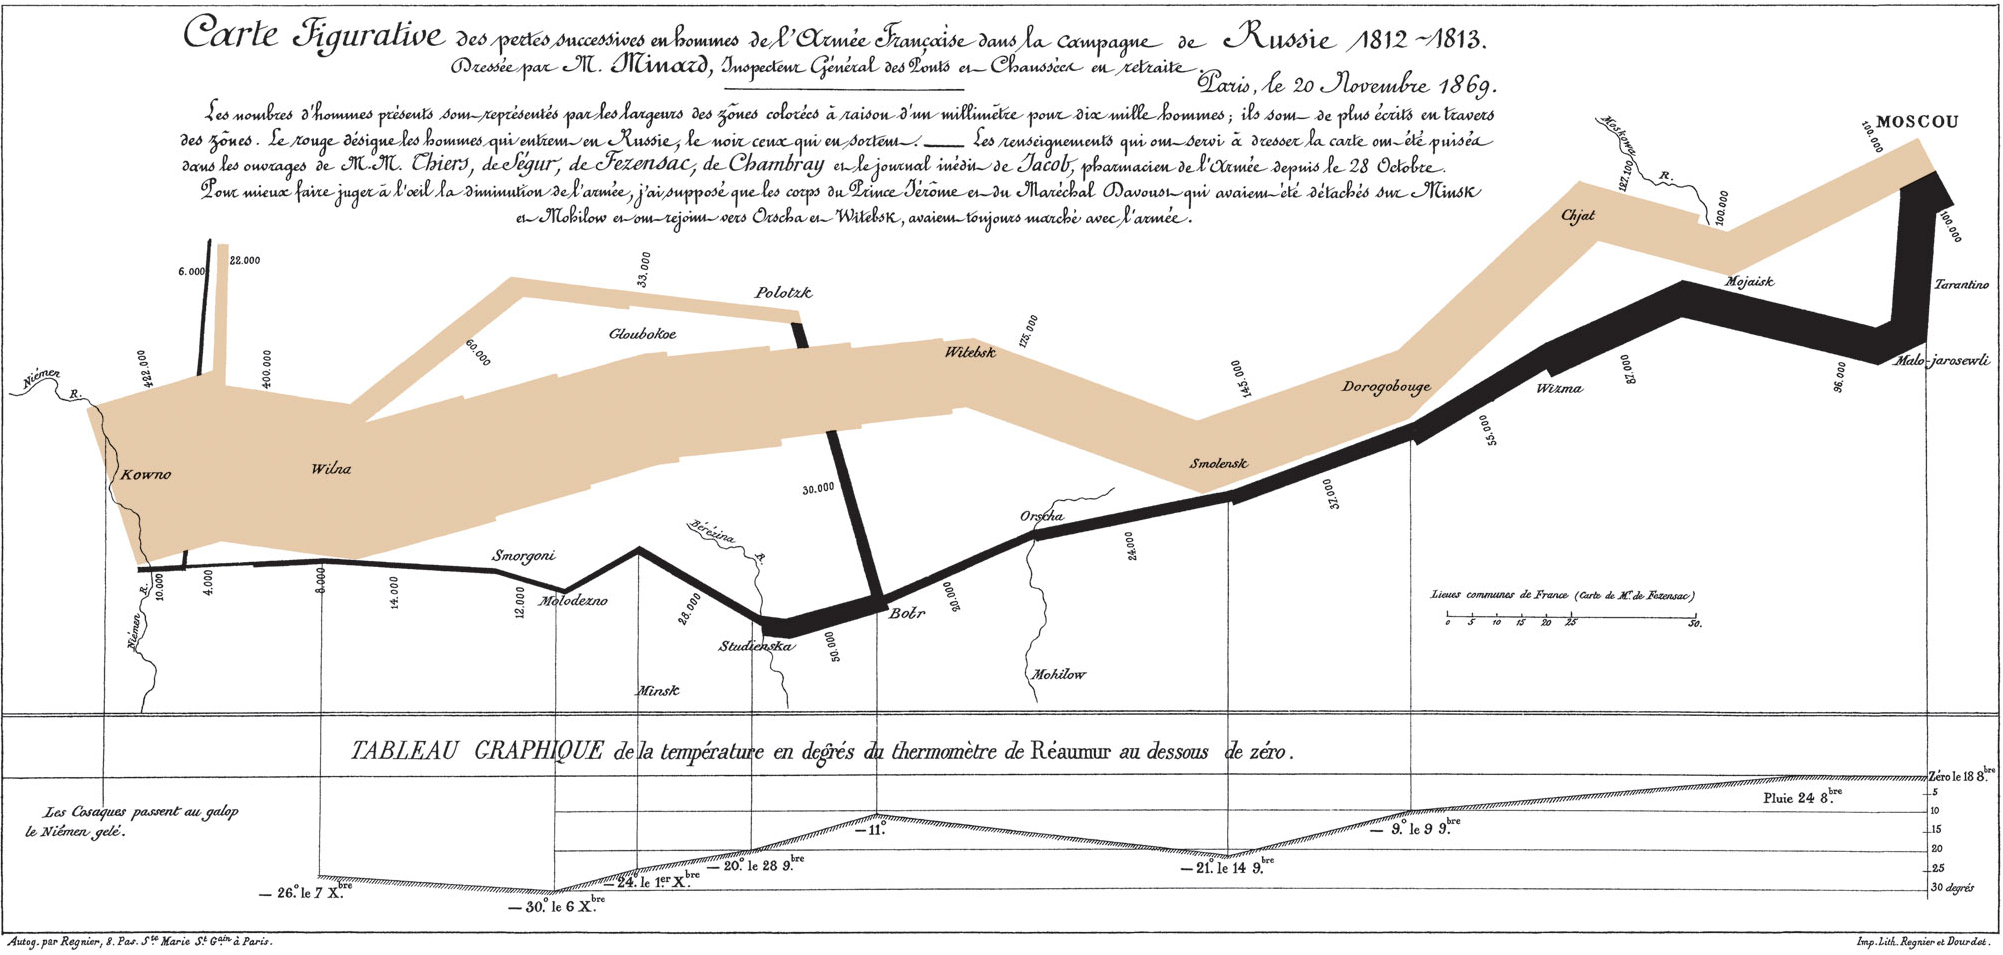
\includegraphics[scale=0.2]{Napoleon2MoscowAndBack}
\par\end{center}

\end{frame}
\ifteacheredition

\begin{frame}{Overview}
\begin{itemize}
\item Edward Tufte: \textquotedblleft the best statistical graphic ever
drawn\textquotedblright{}
\item Six types of information
\begin{itemize}
\item Geography: landmarks and battles
\item Time
\item Temperature: for return journey, along the bottom
\item Course and direction: gold and black
\item Troops remaining: one millimeter for 10,000 men
\end{itemize}
\item Source: \href{https://datavizblog.com/2013/05/26/dataviz-history-charles-minards-flow-map-of-napoleons-russian-campaign-of-1812-part-5/}{datavizblog}
\end{itemize}
\end{frame}
\fi

\begin{frame}{Cholera Outbreak}
\begin{center}
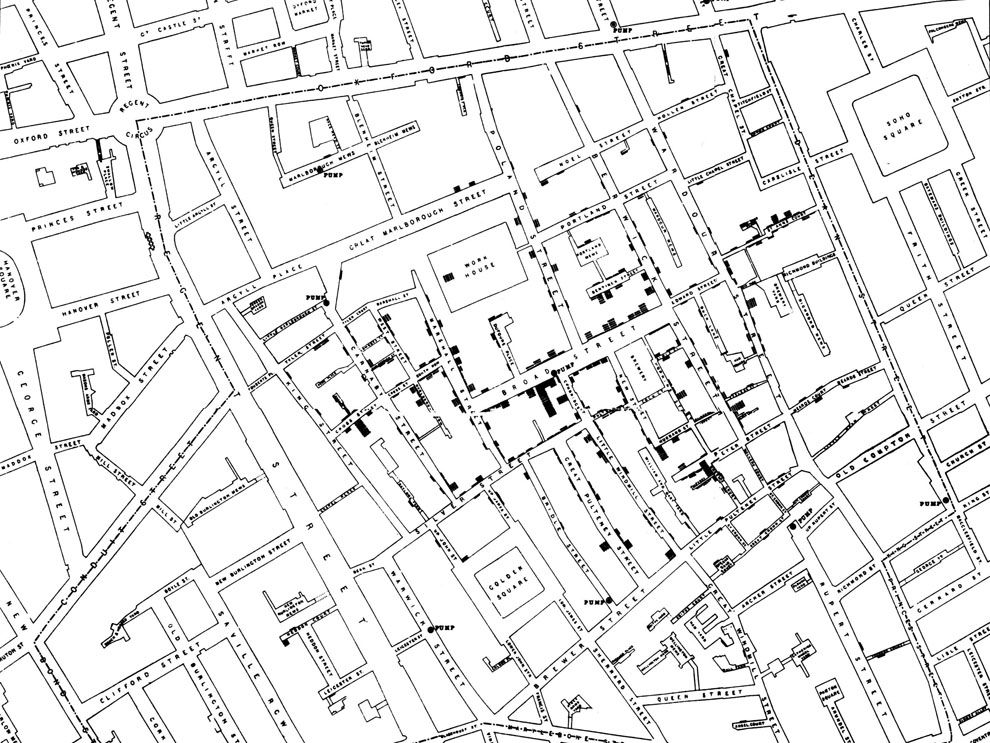
\includegraphics[scale=0.2]{CholeraOutbreakLondon}
\par\end{center}

\end{frame}
\ifteacheredition

\begin{frame}{Overview}
\begin{itemize}
\item Cholera in London's Soho : 
\begin{itemize}
\item Believed to be spread by unpleasant vapor
\item Germs were not yet understood
\item Sudden and serious outbreak was a mystery.
\end{itemize}
\item John Snow (the original) mapped cases and identified a cluster around
the pump in Broad (now Broadwick) street
\begin{itemize}
\item Outliers were asked to link up to the area
\item Close workhouses had own water supply
\end{itemize}
\item Source: \href{https://www.theguardian.com/news/datablog/2013/mar/15/john-snow-cholera-map}{The Guardian}
\end{itemize}
\end{frame}
\fi

\begin{frame}{Contemporary Masterpiece}
\begin{center}
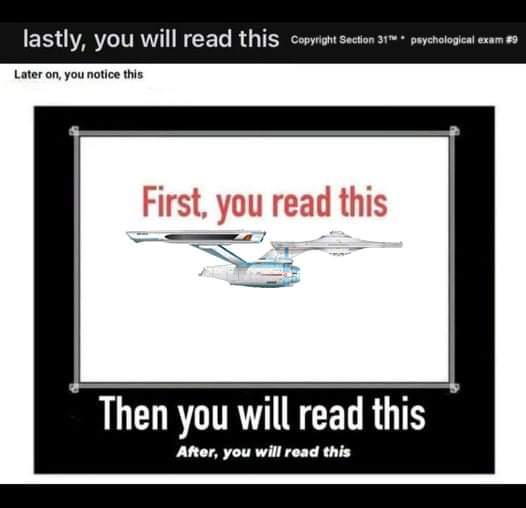
\includegraphics[scale=0.35]{FB_IMG_1631042584438}
\par\end{center}

\end{frame}
%

\section{Objective}
\begin{frame}{Objective}
\begin{center}
Visualize important data concerning international trade in the widest
sense.
\par\end{center}

\end{frame}
\ifteacheredition

\begin{frame}{Visualization}
\begin{center}
\textbf{\emph{Visualize}} important data concerning international
trade in the widest sense.
\par\end{center}
\begin{itemize}
\item Important toolkit in debates, 
\begin{itemize}
\item big data 
\item social media. 
\end{itemize}
\item What is data visualization? 
\end{itemize}
\begin{quotation}
A {[}data{]} visualization is any visual display intended to reveal
evidence, making the invisible visible. 
\begin{quotation}
Alberto Cairo (2015) 
\end{quotation}
\end{quotation}
\begin{itemize}
\item First part: a definition
\begin{itemize}
\item I will not accept an audio file. 
\end{itemize}
\item Second part: an aim
\end{itemize}
\begin{center}
\textbf{Your goal is to point something out!}
\par\end{center}

\end{frame}
%
\begin{frame}{Relevancy}
\begin{center}
Visualize \textbf{\emph{important}} data concerning international
trade in the widest sense.
\par\end{center}
\begin{itemize}
\item Audience
\begin{itemize}
\item Large
\item Important
\end{itemize}
\item issue
\begin{itemize}
\item Costly
\item Unnecessary
\end{itemize}
\item transmission
\begin{itemize}
\item Understandable display
\item Comprehensible message
\end{itemize}
\end{itemize}
\end{frame}
%
\begin{frame}{International}
\begin{center}
Visualize important data concerning \textbf{\emph{international}}\textbf{
}\textbf{\emph{trade}}\textbf{ }in the widest sense.
\par\end{center}
\begin{itemize}
\item Anything that affects cross-country trade. 
\begin{itemize}
\item Lecture notes
\item Beyond!
\end{itemize}
\end{itemize}
\end{frame}
%
\begin{frame}{Reach}
\begin{center}
Visualize important data concerning international trade \textbf{\emph{in
the widest sense}}.
\par\end{center}
\begin{itemize}
\item Theoretical relationship
\begin{itemize}
\item Gravity equation
\end{itemize}
\item Immediate living condition
\begin{itemize}
\item Gender differences
\end{itemize}
\item Business concern
\end{itemize}
\end{frame}
\fi


\section{Timeline}
\begin{frame}{Overview}
\begin{center}
\begin{tabular}{l|l||l}
Date & Time & Topic\tabularnewline
\hline 
17th of February & end-of-day & Consult for topic\tabularnewline
\hline 
22nd of February & classroom & Good viz, bad viz, ugly viz\tabularnewline
\hline 
10th of March & end-of-day & Project topic and data submission\tabularnewline
\hline 
22nd of March & classroom & Rough draft\tabularnewline
\hline 
10th of May & classroom & Final submission\tabularnewline
\hline 
\end{tabular}\textbf{}
\par\end{center}

\end{frame}
\ifteacheredition

\begin{frame}{\textbf{Form teams}}
\begin{itemize}
\item Today!
\end{itemize}
\begin{enumerate}
\item I assign teams of 1-3
\item You assign tasks! You will require
\begin{itemize}
\item Communication and scheduling
\item Literature review
\item Data work 
\item Transformation techniques 
\item Decide on visualization forms and execute
\end{itemize}
Not every tasks needs to be done by one member of your team alone!
\end{enumerate}
\end{frame}
%
\begin{frame}{\textbf{Good viz, bad viz, ugly viz}}
\begin{itemize}
\item Find 1 good, 1 bad, and 1 ugly example of data visualizations
\end{itemize}
\begin{enumerate}
\item Write 3-4 sentences for each examples
\item Collect examples and comments in a presentation you give in class
before (or on) the due date.
\end{enumerate}
\end{frame}
%
\begin{frame}{\textbf{Project topic and data submission}}
\begin{itemize}
\item Follow the next steps:
\end{itemize}
\begin{enumerate}
\item Discuss possible topics
\item Verify that data is available
\item Repeat until you found what you were looking for!
\end{enumerate}
Then, 
\begin{enumerate}
\item Write a title for your project, 
\item Outline the general idea in 3-4 sentences, and 
\item Upload the document and the data you will use before (or on) the due
date.
\end{enumerate}
\end{frame}
%
\begin{frame}{\textbf{Rough draft}}
\begin{enumerate}
\item Apply any data transformation and supporting statistics and plot your
data.
\item Present in class before (or on) the due date:
\begin{enumerate}
\item Title of project
\item Display of data
\item Message
\item Targeted audience
\item Why do you think it is important
\item Why do you chose the form of visualization you display. 
\end{enumerate}
\item Receive feedback!
\item Give feedback!
\end{enumerate}
\end{frame}
%
\begin{frame}{\textbf{Final submission}}
\begin{itemize}
\item Email PNG file before (or on) the due date
\item All projects 
\begin{itemize}
\item will be discussed in class
\item graded by your classmates
\end{itemize}
\end{itemize}
Half of your final grade for this project will depend on their grade!
\end{frame}
\fi


\section{Grading criteria}
\begin{frame}{Grading criteria}
\begin{center}
\begin{tabular}{|l|>{\raggedright}p{3.8cm}|>{\raggedright}p{3.5cm}|l|}
\hline 
{\tiny Dimension} & {\tiny Exemplary} & {\tiny Unsatisfactory} & {\tiny Weight}\tabularnewline
\hline 
\hline 
{\tiny Title} & {\tiny descriptive, informative, intriguing} & {\tiny no title} & {\tiny 10\%}\tabularnewline
\hline 
{\tiny Description} & {\tiny efficient use of text elements} & {\tiny display is inexplicable} & {\tiny 10\%}\tabularnewline
\hline 
\hline 
{\tiny Clarity} & {\tiny data is identifiable immediately} & {\tiny choices lead to ambiguous display} & {\tiny 10\%}\tabularnewline
\hline 
{\tiny Support} & {\tiny assist visualization} & {\tiny data clutter} & {\tiny 20\%}\tabularnewline
\hline 
\hline 
{\tiny Accuracy} & {\tiny data is accurately displayed} & {\tiny display deceives the audience} & {\tiny 10\%}\tabularnewline
\hline 
\hline 
{\tiny Appropriateness} & {\tiny display matches message} & {\tiny display does not mirror message} & {\tiny 20\%}\tabularnewline
\hline 
{\tiny Impact} & {\tiny could headline an Economist article} & {\tiny is a waste of time and attention} & {\tiny 20\%}\tabularnewline
\hline 
\hline 
{\tiny Grade} & {\tiny 10} & {\tiny 6} & {\tiny 100\%}\tabularnewline
\hline 
\end{tabular}
\par\end{center}

\end{frame}
%

\section{General advice and examples}

\subsection{General advice}
\begin{frame}[allowframebreaks]{General advice}
\begin{enumerate}
\item Tell a story.
\item ``Show the data'' $\not\Rightarrow$ ``show \emph{all} the data''. 
\begin{itemize}
\item Declutter, and avoid a ``data dump''.
\end{itemize}
\item It is easier to identify objects by color than by shape.
\begin{itemize}
\item Use color intentionally.
\item black-white printouts.
\end{itemize}
\item Don't graph for the author!
\begin{itemize}
\item Data exploration vs conveying a message
\end{itemize}
\item Default graph options in software tends to clutter and separate text
and graphs
\begin{itemize}
\item Add annotations and avoid legends
\item Researcher explore using default grid lines, tick marks, and colors 
\end{itemize}
\item Elements such as text, lines, shapes, etc, that have the same nature
should look alike.
\item Strive for balance between graphic and explanatory text.
\item Prevent your audience from asking ``so what?'' by showing 
\begin{itemize}
\item contrasts, 
\item comparisons, 
\item differences.
\end{itemize}
\item Avoid the third dimension, it is usually not helpful.
\end{enumerate}
\end{frame}
%
\begin{frame}[allowframebreaks]{Specifics}
\begin{enumerate}
\item Data sources should be included in a very brief way.
\item You can use supporting statistics such as filters, trends, etc., to
make your point.
\item I provide some examples with Matlab code.
\begin{itemize}
\item There is no software requirement.
\end{itemize}
\item Some tools and data sources are mentioned in the document ``Data
visualization assignment'' on the webpage of this course.
\item The aforementioned points are suggestions based on my own taste and
experience about prevalent usage. They are not commandments.
\end{enumerate}
\end{frame}
%

\subsection{Schwabish (2014)}

\subsubsection{General}
\begin{frame}{Count the 3s}
 

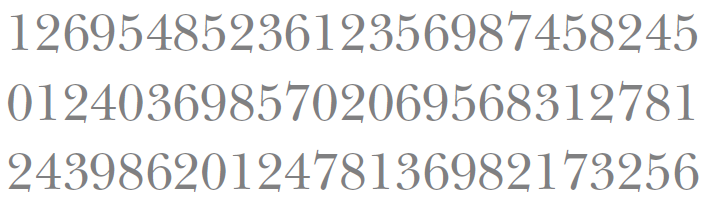
\includegraphics[scale=0.55]{Schwabish2014_1}
\end{frame}
%
\begin{frame}{Count again}

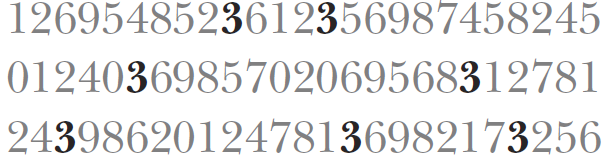
\includegraphics[scale=0.65]{Schwabish2014_2}
\end{frame}
%
\begin{frame}{Pre-attentive visual processing}
\begin{itemize}
\item Attentive processing
\item Pre-attentive processing is done in parallel and faster
\end{itemize}
\end{frame}
%
\ifteacheredition
\begin{frame}{Pre-attentive visual processing}
\begin{itemize}
\item Attentive processing
\begin{itemize}
\item the conscious part of perception that allows us to perceive things
serially
\end{itemize}
\item Pre-attentive processing is done in parallel and faster
\begin{itemize}
\item instances of 3s are easier to find because they are encoded using
a different pre-atttentive attribute
\item intensity of boldface type.
\end{itemize}
\end{itemize}
\end{frame}
%
\fi
\begin{frame}{Picture Superiority Effect}
\begin{itemize}
\item Our ability to retain information from pictures exceeds the ability
to do the same through words
\end{itemize}
\end{frame}
%
\begin{frame}{Declutter}
\begin{center}
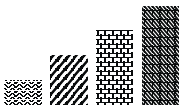
\includegraphics[scale=0.7]{Schwabish2014_3} and 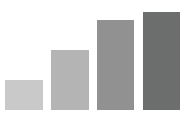
\includegraphics[scale=0.7]{Schwabish2014_4} 
\par\end{center}

\begin{center}
display the same information.
\par\end{center}

\end{frame}
%

\subsubsection{Line chart}
\begin{frame}{Original}
\begin{center}
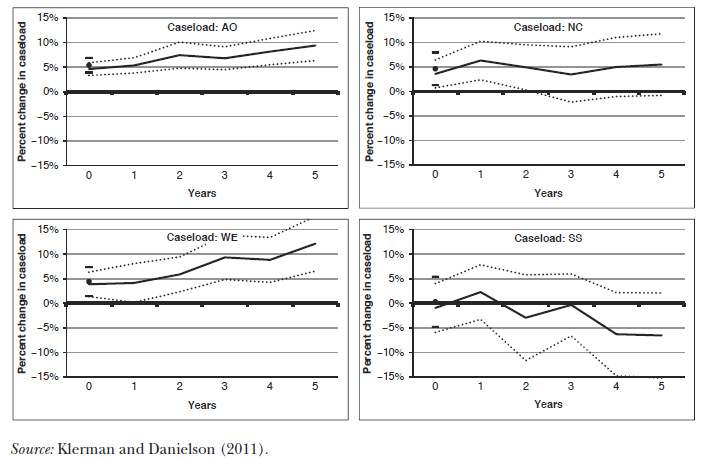
\includegraphics[scale=0.55]{Schwabish2014_5}
\par\end{center}

\end{frame}
\begin{center}
\ifteacheredition
\par\end{center}

\begin{frame}{Message}
\begin{itemize}
\item Klerman and Danielson (2011)
\item Message: regression results of the correlation between the long-run
unemployment rate in the United States and Supplemental Nutrition
Assistance Program caseloads for four�groups
\item Instead of single line: four smaller charts combined
\begin{itemize}
\item Not a bad idea
\end{itemize}
\end{itemize}
\end{frame}
%
\begin{frame}{Critique}
\begin{enumerate}
\item The darkest and thickest line is the 0�percent grid line.
\begin{itemize}
\item not the data!
\end{itemize}
\item Some data values exceed the upper bound of the chart
\item Clutter:
\begin{itemize}
\item The y-axis labels and percentage signs are redundant 
\begin{itemize}
\item 28�percentage signs in�total!
\end{itemize}
\item Tick marks on the y-axes are unnecessary.
\end{itemize}
\item What do AO, NC, WE, and SS mean?
\begin{itemize}
\item Terms are explained on the third and fourth�pages, 15�pages before
this figure
\end{itemize}
\end{enumerate}
\end{frame}
\fi

\begin{frame}{Revision}
\begin{center}
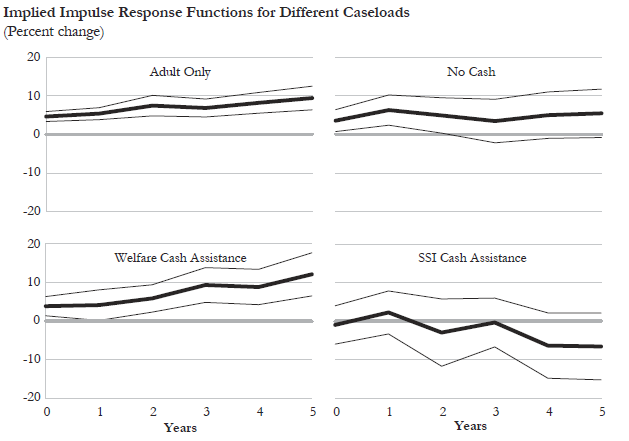
\includegraphics[scale=0.6]{Schwabish2014_5b}
\par\end{center}

\end{frame}
\begin{center}
\ifteacheredition
\par\end{center}

\begin{frame}{Improvement}
\begin{itemize}
\item The darkest line shows the data
\item The grid lines are lighter
\begin{itemize}
\item leaving the 0�percent grid line darker as a reference. 
\end{itemize}
\item Two�sets of labels are gone
\begin{itemize}
\item The charts are aligned vertically and horizontally 
\end{itemize}
\item Percent signs are gone 
\begin{itemize}
\item Units are below the title
\end{itemize}
\item y-label moved to the title
\begin{itemize}
\item Rotated text on the vertical axis requires readers to turn the page
sideways or tilt their heads 
\end{itemize}
\item The title is now above the graph
\begin{itemize}
\item Readers tend to start reading from the top left, move down along the
left margin, and then move to the right.
\end{itemize}
\item \textquotedblleft Caseload\textquotedblright{} moves into the title
\begin{itemize}
\item used four�times in the original
\end{itemize}
\item Abbreviations are spelled out
\end{itemize}
\end{frame}
\fi


\subsubsection{Clutterplot}
\begin{frame}{Original}
\begin{center}
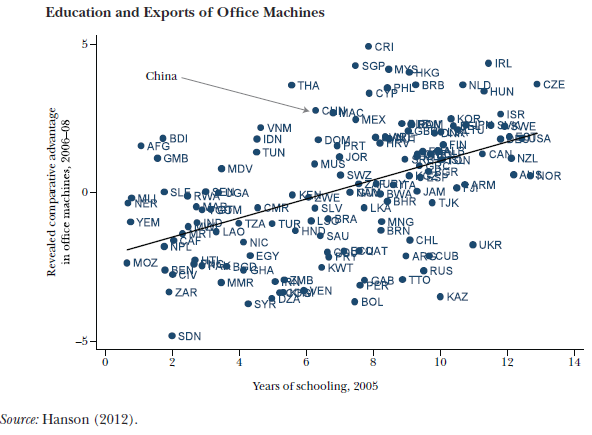
\includegraphics[scale=0.6]{Schwabish2014_6}
\par\end{center}

\end{frame}
\begin{center}
\ifteacheredition
\par\end{center}

\begin{frame}{Message}
\begin{itemize}
\item Hanson (2012, JEP)
\item ``{[}The figure{]} plots countries\textquoteright{} revealed comparative
advantage in office machines . . . averaged over 2006 to 2008, against
the average years of schooling of the adult population in 2005 . .
. China is above the regression line, indicating that its specialization
in the sector is greater than one would expect given its level of
education, but it is hardly an extreme outlier. Other middle-income
countries---including Costa Rica, the Philippines, Malaysia, and
Thailand---have larger positive residuals.''
\end{itemize}
\end{frame}
%
\begin{frame}{Critique}
\begin{itemize}
\item Do you know the 3 letter code for China, Costa Rica, the Philippines,
Malaysia, and Thailand?
\end{itemize}
\end{frame}
\fi

\begin{frame}{Revision}
\begin{center}
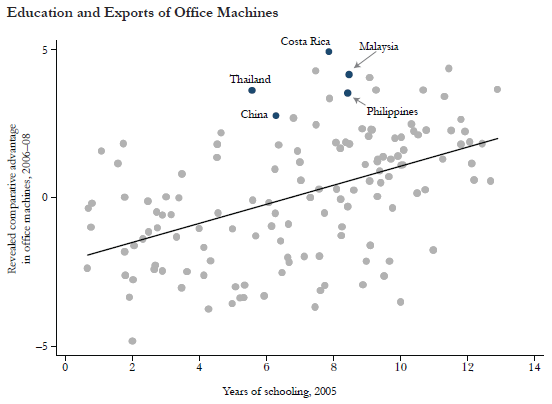
\includegraphics[scale=0.65]{Schwabish2014_6b}
\par\end{center}

\end{frame}
\begin{center}
\ifteacheredition
\par\end{center}

\begin{frame}{Improvement}
\begin{itemize}
\item Eliminate all but 5 relevant countries and spell out those.
\begin{itemize}
\item Conflict: some reader might want to know about individual countries
or identify outliers.
\begin{itemize}
\item Classic trade-off
\item supplemental table or data provision
\end{itemize}
\end{itemize}
\end{itemize}
\end{frame}
\fi


\subsubsection{Column Chart}
\begin{frame}{Intermezzo}
\begin{center}
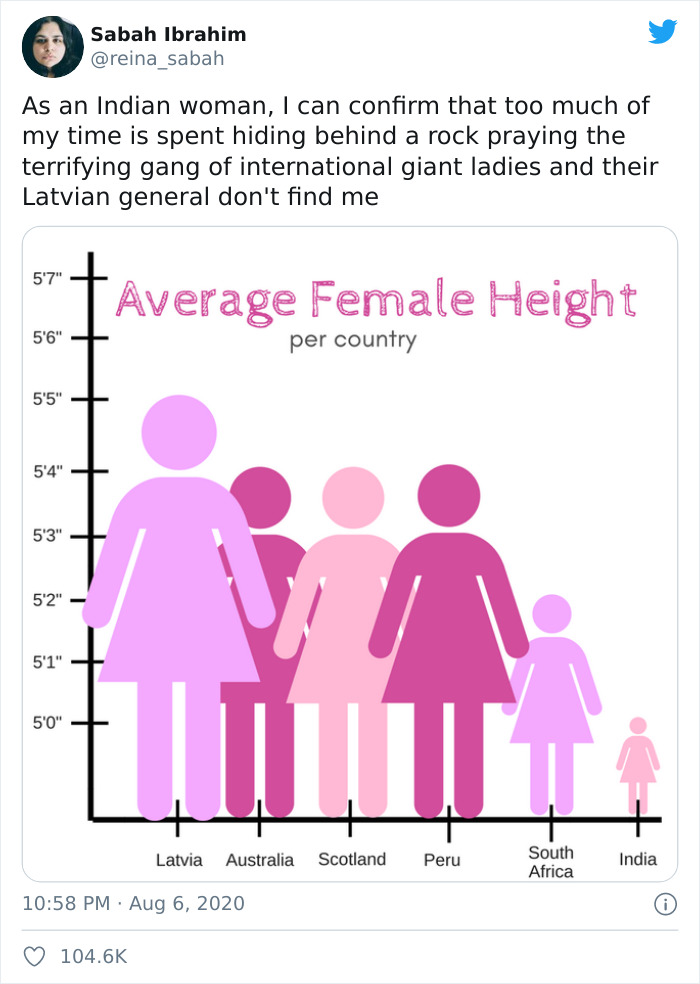
\includegraphics[scale=0.2]{FemaleHeight}
\par\end{center}

\end{frame}
%
\begin{frame}{Original}
\begin{center}
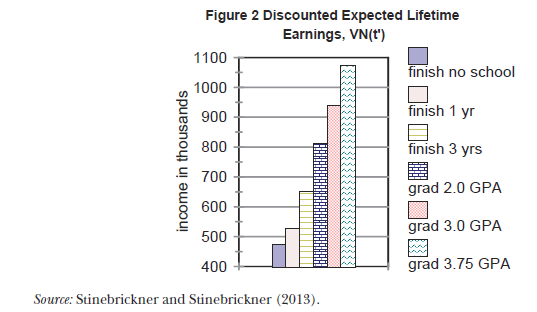
\includegraphics[scale=0.65]{Schwabish2014_7}
\par\end{center}

\begin{center}
Are discounted expected lifetime earnings of someone with 1 year of
schooling half of those finishing with a 3.75 GPA?
\par\end{center}

\end{frame}
\begin{center}
\ifteacheredition
\par\end{center}

\begin{frame}{Critique}
\begin{itemize}
\item My eyes say no!
\item Different colors/patterns for each bar - why?
\begin{itemize}
\item visual matching using a legend
\end{itemize}
\end{itemize}
\end{frame}
\fi

\begin{frame}{Revision}
\begin{center}
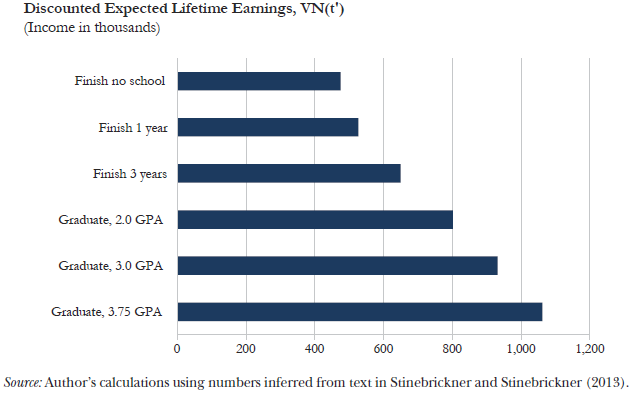
\includegraphics[scale=0.6]{Schwabish2014_7B}
\par\end{center}

\end{frame}
\begin{center}
\ifteacheredition
\par\end{center}

\begin{frame}{Improvement}
\begin{itemize}
\item The axis starts at zero
\item The figure is rotated horizontally 
\begin{itemize}
\item to make room for the labels
\end{itemize}
\item Finish 1 year vs grad 3.75 GPA appear comparable
\end{itemize}
\end{frame}
\fi


\subsubsection{3D Chart}
\begin{frame}{Original}
\begin{center}
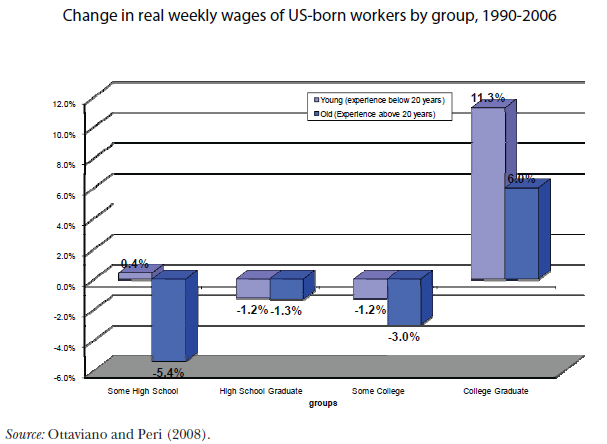
\includegraphics[scale=0.55]{Schwabish2014_8}
\par\end{center}

\end{frame}
\begin{center}
\ifteacheredition
\par\end{center}

\begin{frame}{Critique}
\begin{itemize}
\item Third�dimension 
\begin{itemize}
\item does not plot data values
\item adds clutter to the chart 
\item distorts the information.
\begin{itemize}
\item far-right-hand bar, labeled 6�percent, does not touch gridline
\end{itemize}
\end{itemize}
\end{itemize}
\end{frame}
\fi

\begin{frame}{Revision}
\begin{center}
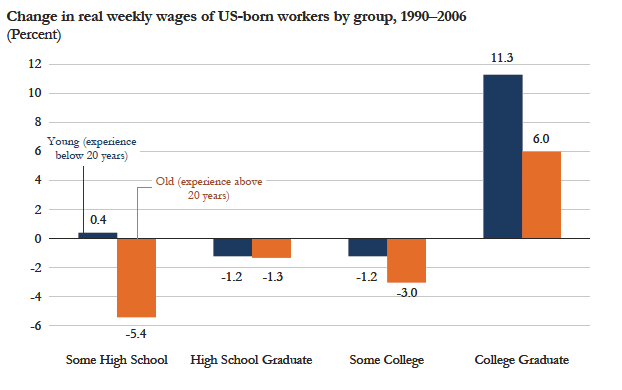
\includegraphics[scale=0.65]{Schwabish2014_8b}
\par\end{center}

\end{frame}
\begin{center}
\ifteacheredition
\par\end{center}

\begin{frame}{Improvement}
\begin{itemize}
\item Cancel the 3D�treatment 
\item Integrate the disconnected legend with the graph. 
\item Common baseline permits an effective comparison
\begin{itemize}
\item was portrayed by a hovering, barely perceptible thin gray line
\end{itemize}
\end{itemize}
\end{frame}
\fi


\subsubsection{Unbalanced Chart}
\begin{frame}{Original}
\begin{center}
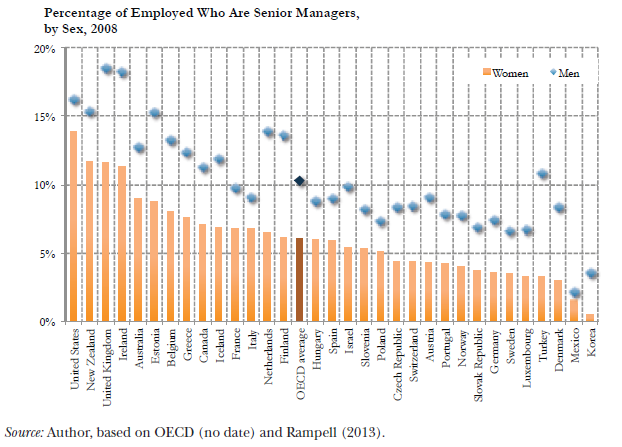
\includegraphics[scale=0.6]{Schwabish2014_9}
\par\end{center}

\end{frame}
\begin{center}
\ifteacheredition
\par\end{center}

\begin{frame}{Source}
\begin{itemize}
\item Organisation for Economic Co-operation and Development
\item later reproduced in a New York Times Economix blog post
\end{itemize}
\end{frame}
%
\begin{frame}{Critique}
\begin{itemize}
\item Same kinds of data are plotted using different types of encoding 
\begin{itemize}
\item diamonds and bars
\end{itemize}
\item The men are too far away from the women without visual connection
\item The columns for women take up a large proportion, overemphasizing
the data for women.
\begin{itemize}
\item Focus on women? Then change the title: \textquotedblleft Women\textquoteright s
Employment as Senior Managers Averaged 6 Percent in 2008\textquotedblright{}
\end{itemize}
\item Too many grid lines
\item The percent signs on the y-axis labels are redundant. 
\item X-axis labels are potentially difficult to scan because they are vertical.
\end{itemize}
\end{frame}
\fi

\begin{frame}{Revision}
\begin{center}
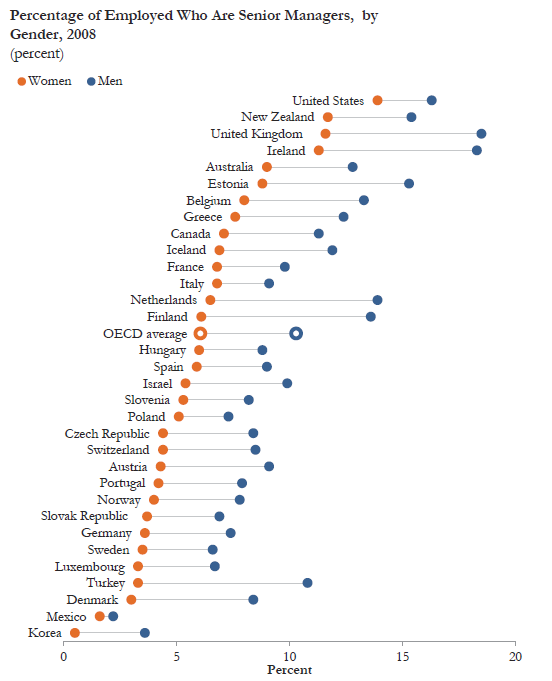
\includegraphics[scale=0.37]{Schwabish2014_9b}
\par\end{center}

\end{frame}
\begin{center}
\ifteacheredition
\par\end{center}

\begin{frame}{Improvement}
\begin{itemize}
\item Visualization a bit ``exotic''
\item Data is encoded similarly for men and women
\begin{itemize}
\item dots
\end{itemize}
\item Thin gray lines connecting the two�series enhances comparison 
\begin{itemize}
\item men vs women
\item different countries
\end{itemize}
\item The title, units, and legend are summarily placed at the top-left
so the reader can \textquotedblleft enter\textquotedblright{} the
chart there.
\item The country labels are rotated horizontally and incorporated next
to the observation
\item The average value for the OECD as a whole is an unfilled circle
\begin{itemize}
\item helps printing gray scale
\end{itemize}
\item Shortcoming: no vertical lines!
\end{itemize}
\end{frame}
\fi


\subsubsection{Spaghetti Chart}
\begin{frame}{Original}
\begin{center}
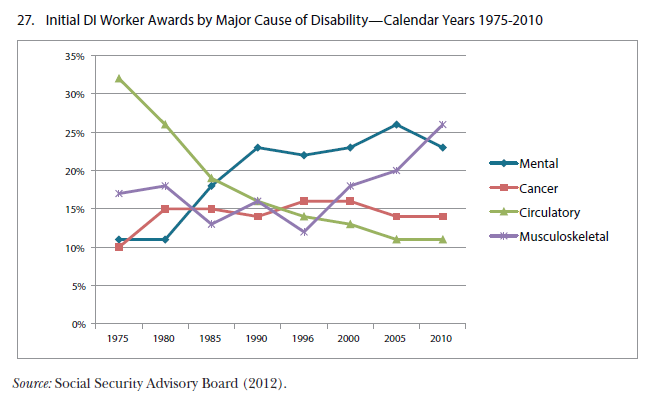
\includegraphics[scale=0.6]{Schwabish2014_10}
\par\end{center}

\end{frame}
\begin{center}
\ifteacheredition
\par\end{center}

\begin{frame}{Critique}
\begin{itemize}
\item the legend 
\begin{itemize}
\item is far from the data 
\item the order of the legend does not match the order of the lines.
\end{itemize}
\item Spaghetti charts, in general, overwhelm if it contains more than,
say, 4 lines.
\end{itemize}
\end{frame}
\fi

\begin{frame}{Revision}
\begin{center}
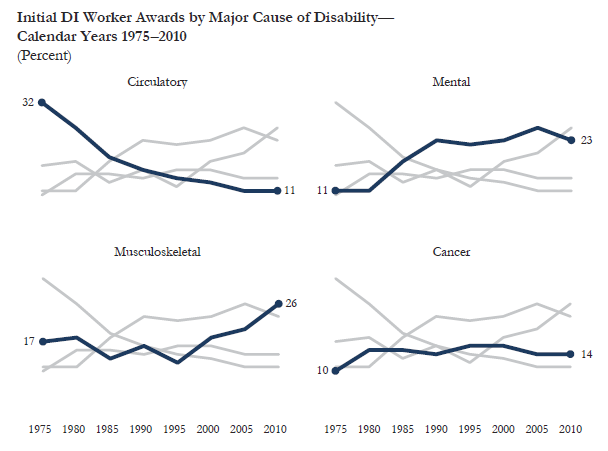
\includegraphics[scale=0.6]{Schwabish2014_10b}
\par\end{center}

\end{frame}
\begin{center}
\ifteacheredition
\par\end{center}

\begin{frame}{Improvement}
\begin{itemize}
\item Create smaller charts in series
\begin{itemize}
\item Highlights the trend in each line
\item Without loosing comparison 
\item While reducing clutter
\end{itemize}
\item Recycle y-axis labels
\end{itemize}
\end{frame}
\fi


\subsubsection{Pie Chart}
\begin{frame}{Size order}
\begin{center}
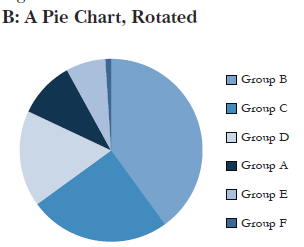
\includegraphics[scale=0.8]{Schwabish2014_pieB}
\par\end{center}

\begin{center}
What is the fraction of group C?
\par\end{center}

\end{frame}
%
\begin{frame}{Alphabetical order}
\begin{center}
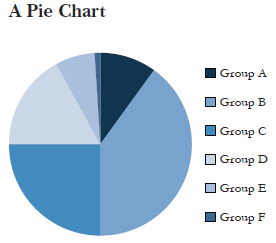
\includegraphics[scale=0.8]{Schwabish2014_pieA}
\par\end{center}

\begin{center}
Obviously 25\%! So, order matters!
\par\end{center}

\begin{center}
What about the rest?
\par\end{center}

\end{frame}
%
\begin{frame}{Size, labeled}
\begin{center}
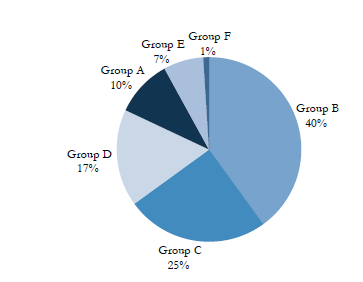
\includegraphics[scale=0.9]{Schwabish2014_pieC}
\par\end{center}

\end{frame}
\begin{center}
\ifteacheredition
\par\end{center}

\begin{frame}{Statistical pie is not apple pie is not }
\begin{itemize}
\item Comparison of areas is actually difficult
\begin{itemize}
\item worse for Donut chart where center (with angles) is missing
\end{itemize}
\end{itemize}
\end{frame}
\fi

\begin{frame}{Alternative}
\begin{center}
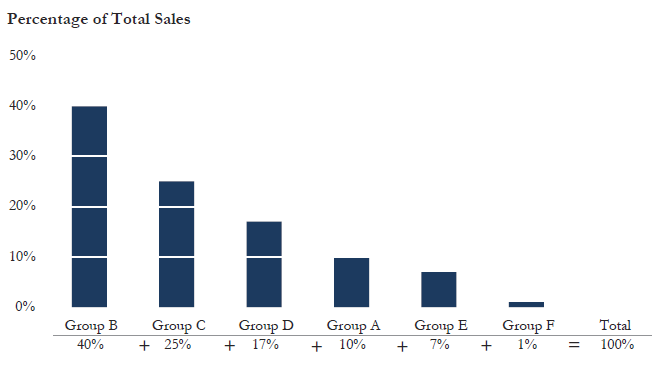
\includegraphics[scale=0.6]{Schwabish2014_pieAlternative}
\par\end{center}

\begin{center}
Size comparison immediately accessible.
\par\end{center}

\end{frame}
%
\begin{frame}{Alternative 2}
\begin{center}
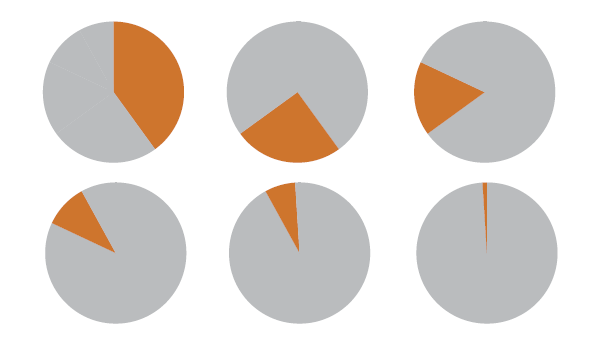
\includegraphics[scale=0.62]{Schwabish2014_pieAlternative2}
\par\end{center}
\begin{itemize}
\item recover ``part-of-a-whole'' comparison while size-comparison is
preserved
\end{itemize}
\end{frame}
%
\begin{frame}{An original pie chart}
\begin{center}
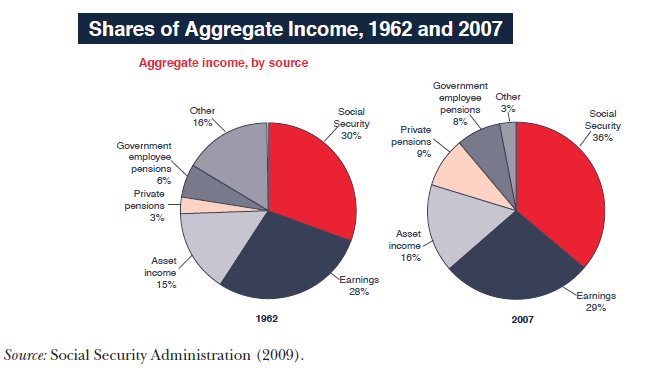
\includegraphics[scale=0.65]{Schwabish2014_11}
\par\end{center}

\end{frame}
\begin{center}
\ifteacheredition
\par\end{center}

\begin{frame}{Intention}
\begin{itemize}
\item Comparison not just 
\begin{itemize}
\item part-of-a-whole
\item between different parts
\end{itemize}
but also over time!
\end{itemize}
\end{frame}
\fi

\begin{frame}{Revision}
\begin{center}
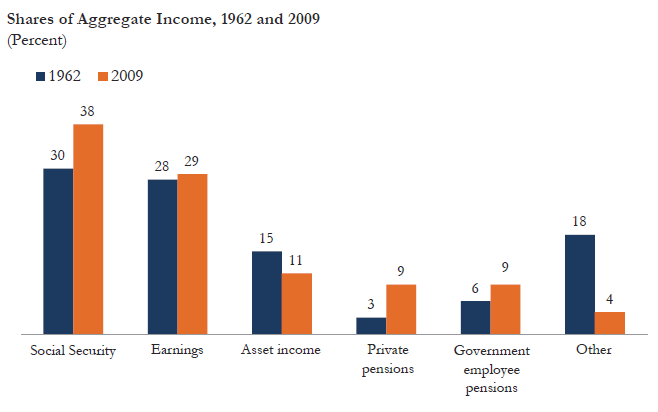
\includegraphics[scale=0.62]{Schwabish2014_11b}
\par\end{center}

\end{frame}
\begin{center}
\ifteacheredition
\par\end{center}

\begin{frame}{Improvement}
\begin{itemize}
\item This is called \emph{paired column chart }
\begin{itemize}
\item fosters within-category/over-time comparisons.
\end{itemize}
\item Y-axis is omitted
\item Few observations allow for vertical orientation
\end{itemize}
\end{frame}
\fi

\begin{frame}{Another revision}
\begin{center}
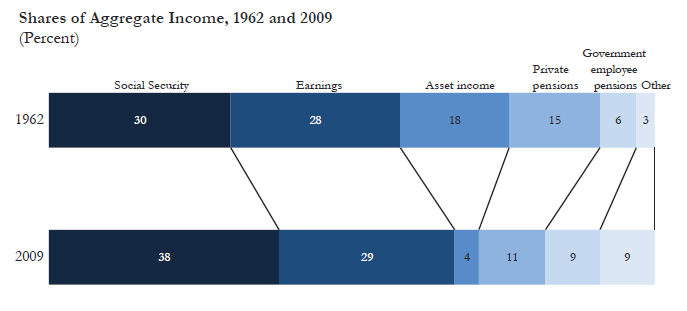
\includegraphics[scale=0.6]{Schwabish2014_11c}
\par\end{center}

\end{frame}
\begin{center}
\ifteacheredition
\par\end{center}

\begin{frame}{Improvement}
\begin{itemize}
\item This is called \emph{stacked bar chart}
\item Shows 
\begin{itemize}
\item the distribution of the various groups 
\item the groups sum to 100�percent
\item changes over time
\end{itemize}
\end{itemize}
\end{frame}
\fi

\begin{frame}{Yet another revision}
\begin{center}
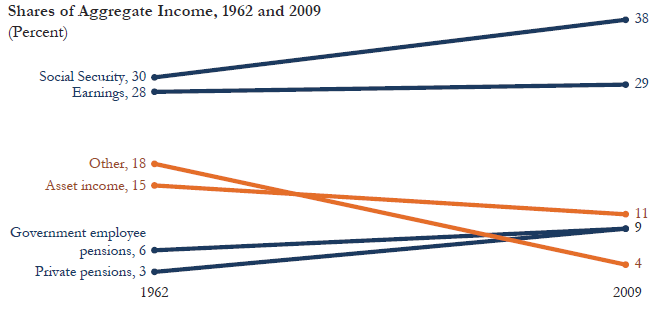
\includegraphics[scale=0.65]{Schwabish2014_11d}
\par\end{center}

\end{frame}
\begin{center}
\ifteacheredition
\par\end{center}

\begin{frame}{Improvement}
\begin{itemize}
\item This is called \emph{slope chart}
\item Shows 
\begin{itemize}
\item the size-order
\item changes over time
\end{itemize}
\end{itemize}
\end{frame}
\fi


\subsection{Liquid Mexico}

\ifteacheredition
\begin{frame}{My own motivation}
\begin{itemize}
\item I would like to engage more over social media
\item But note: my examples are very low tech in terms of support!
\end{itemize}
\end{frame}
%
\fi
\begin{frame}{Lets try one:}
\begin{center}
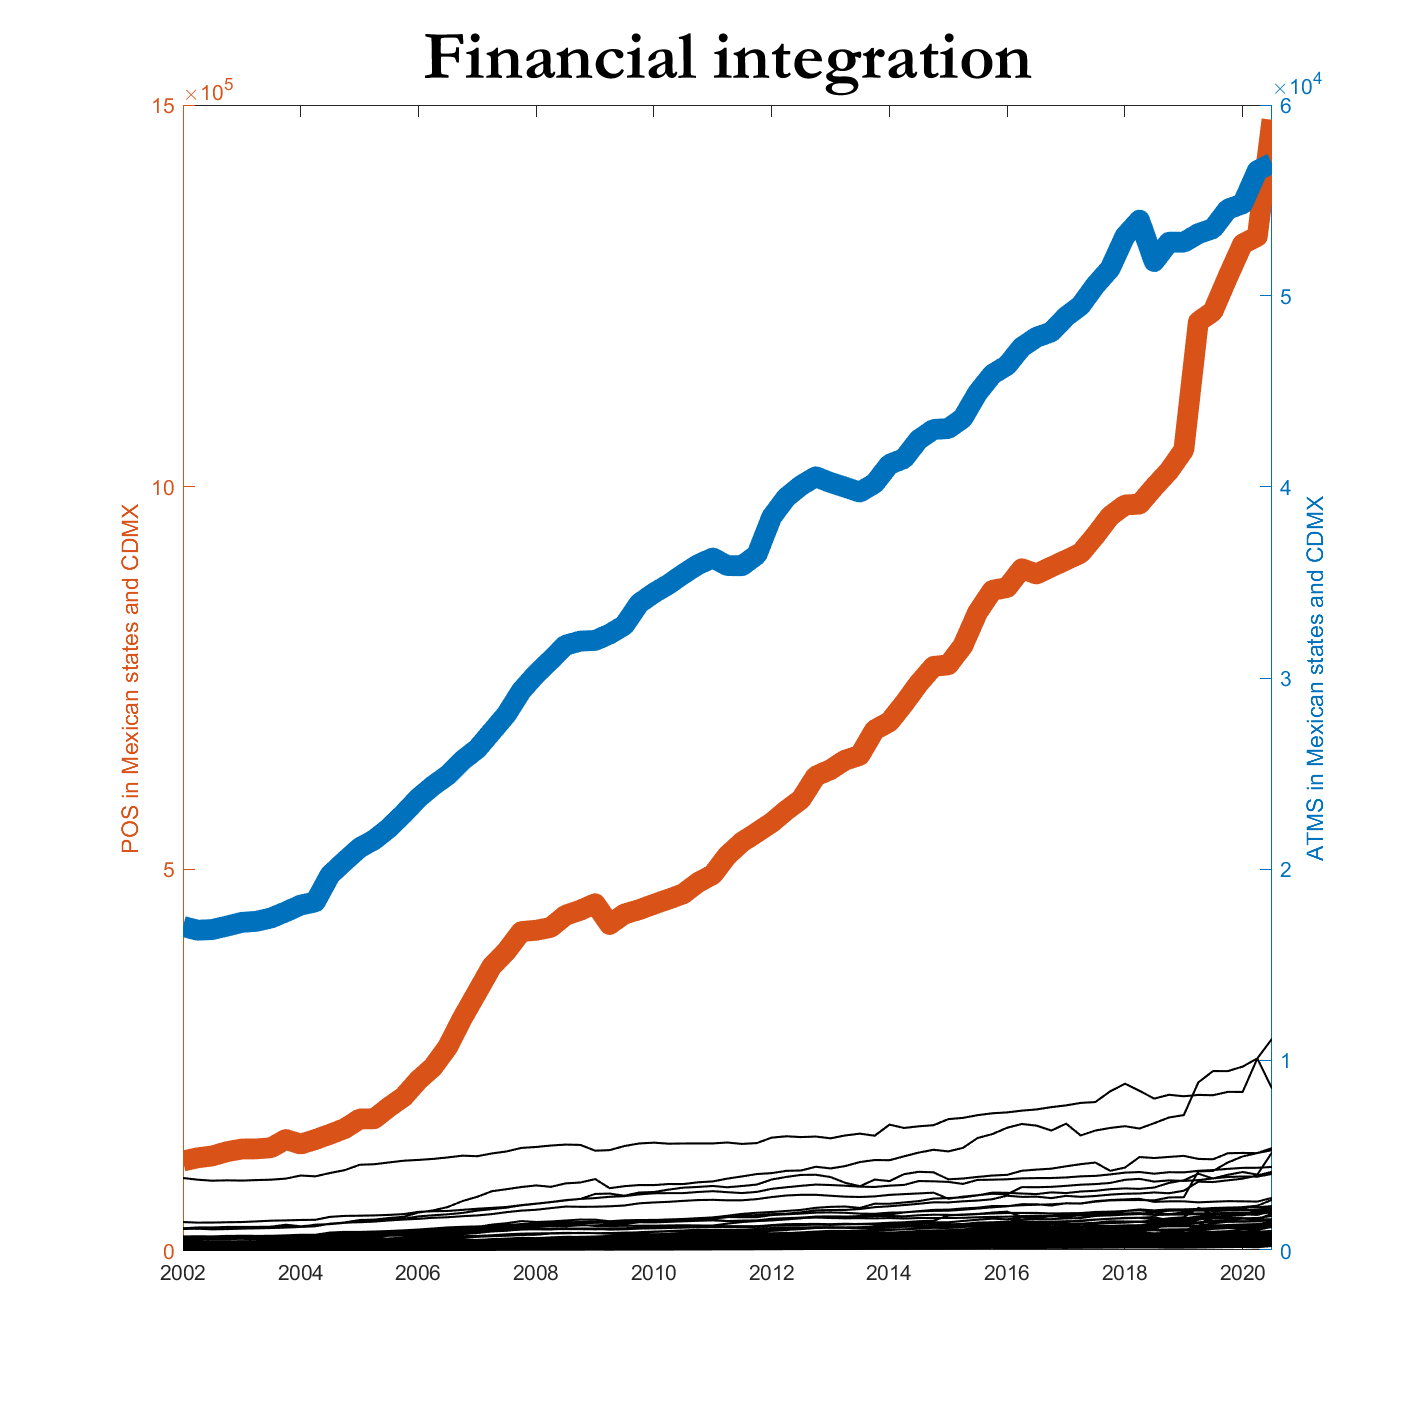
\includegraphics[scale=0.3]{LM_POSvsATMS_BAD}
\par\end{center}

\end{frame}
%
\begin{frame}{An improvement}
\begin{center}
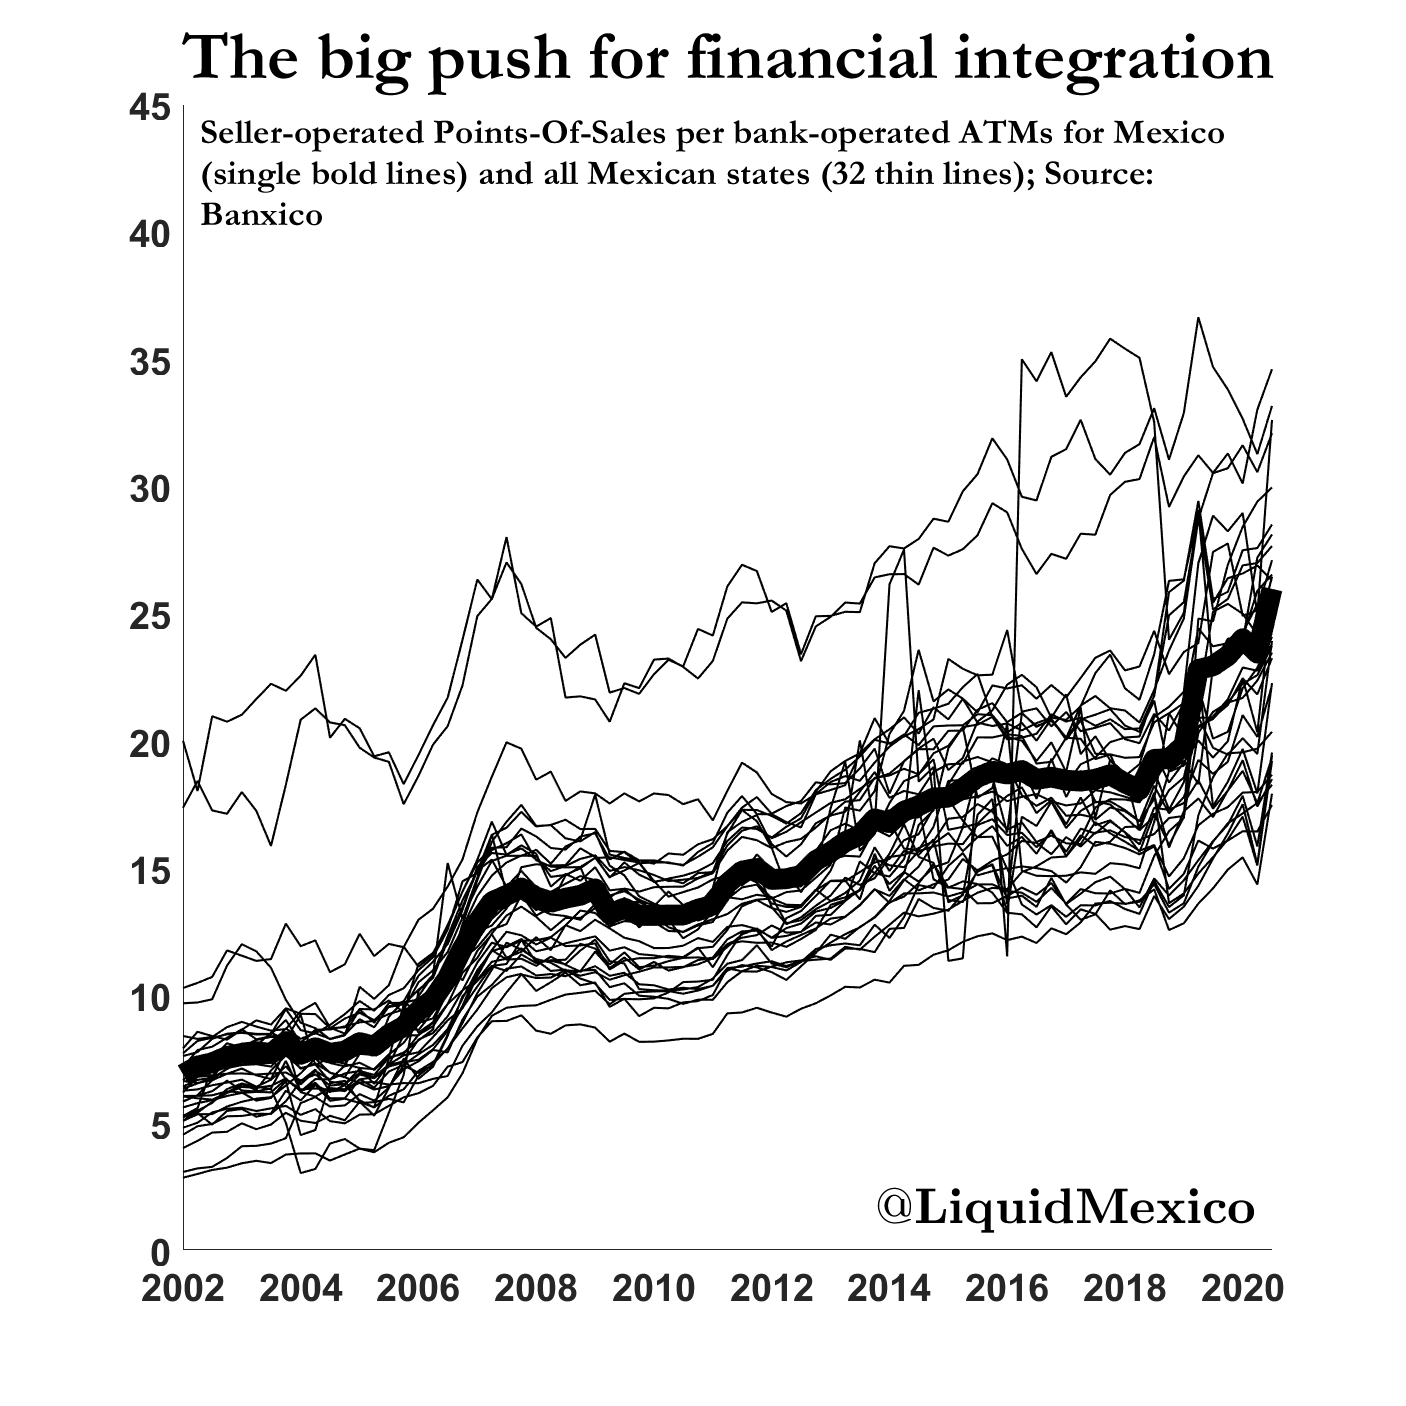
\includegraphics[scale=0.3]{LM_POSvsATMS}
\par\end{center}

\end{frame}
%
\begin{frame}{Another attempt}
\begin{center}
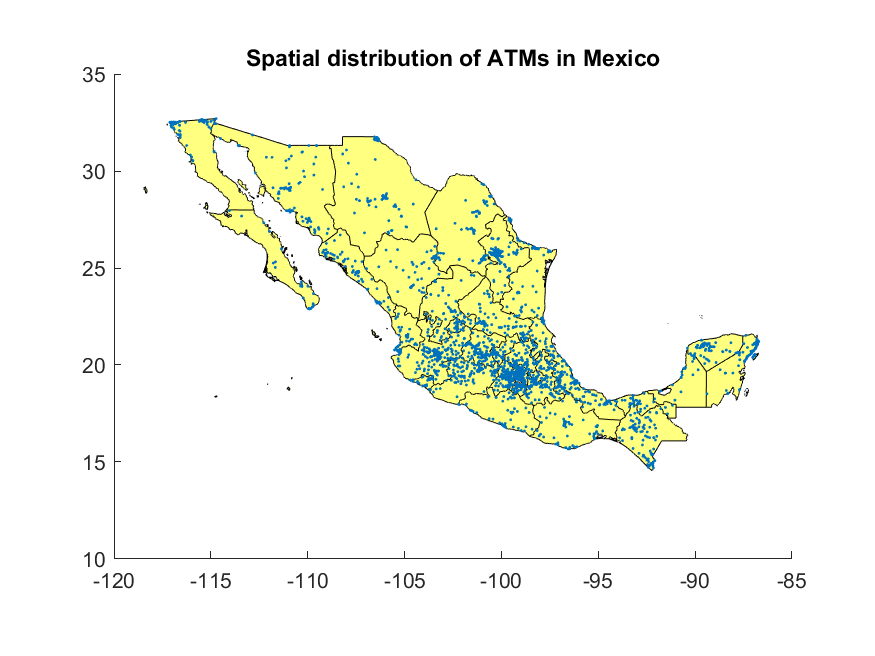
\includegraphics[scale=0.58]{LM_ATMsAndRoadsCDMX_BAD}
\par\end{center}

\end{frame}
%
\begin{frame}{Another revision}
\begin{center}
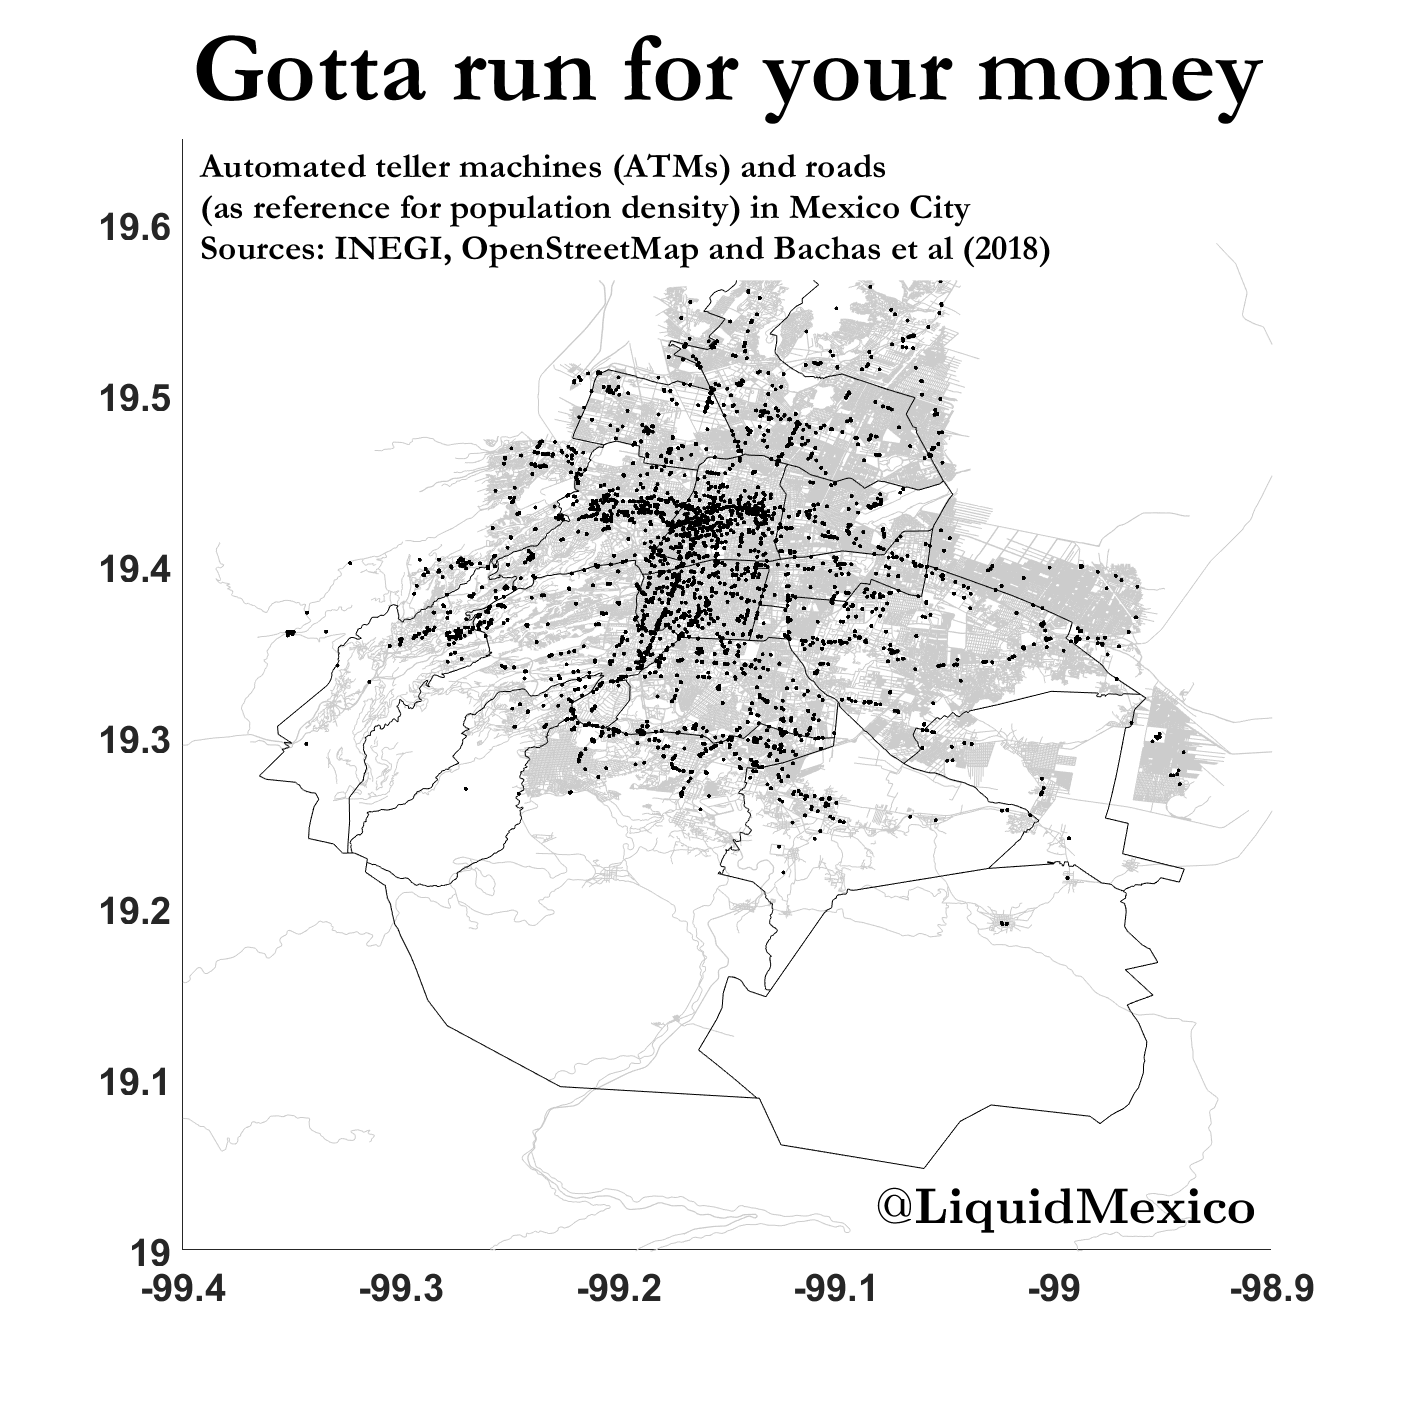
\includegraphics[scale=0.28]{LM_ATMsAndRoadsCDMX}
\par\end{center}

\end{frame}
%
\begin{frame}{Yet another attempt}
\begin{center}
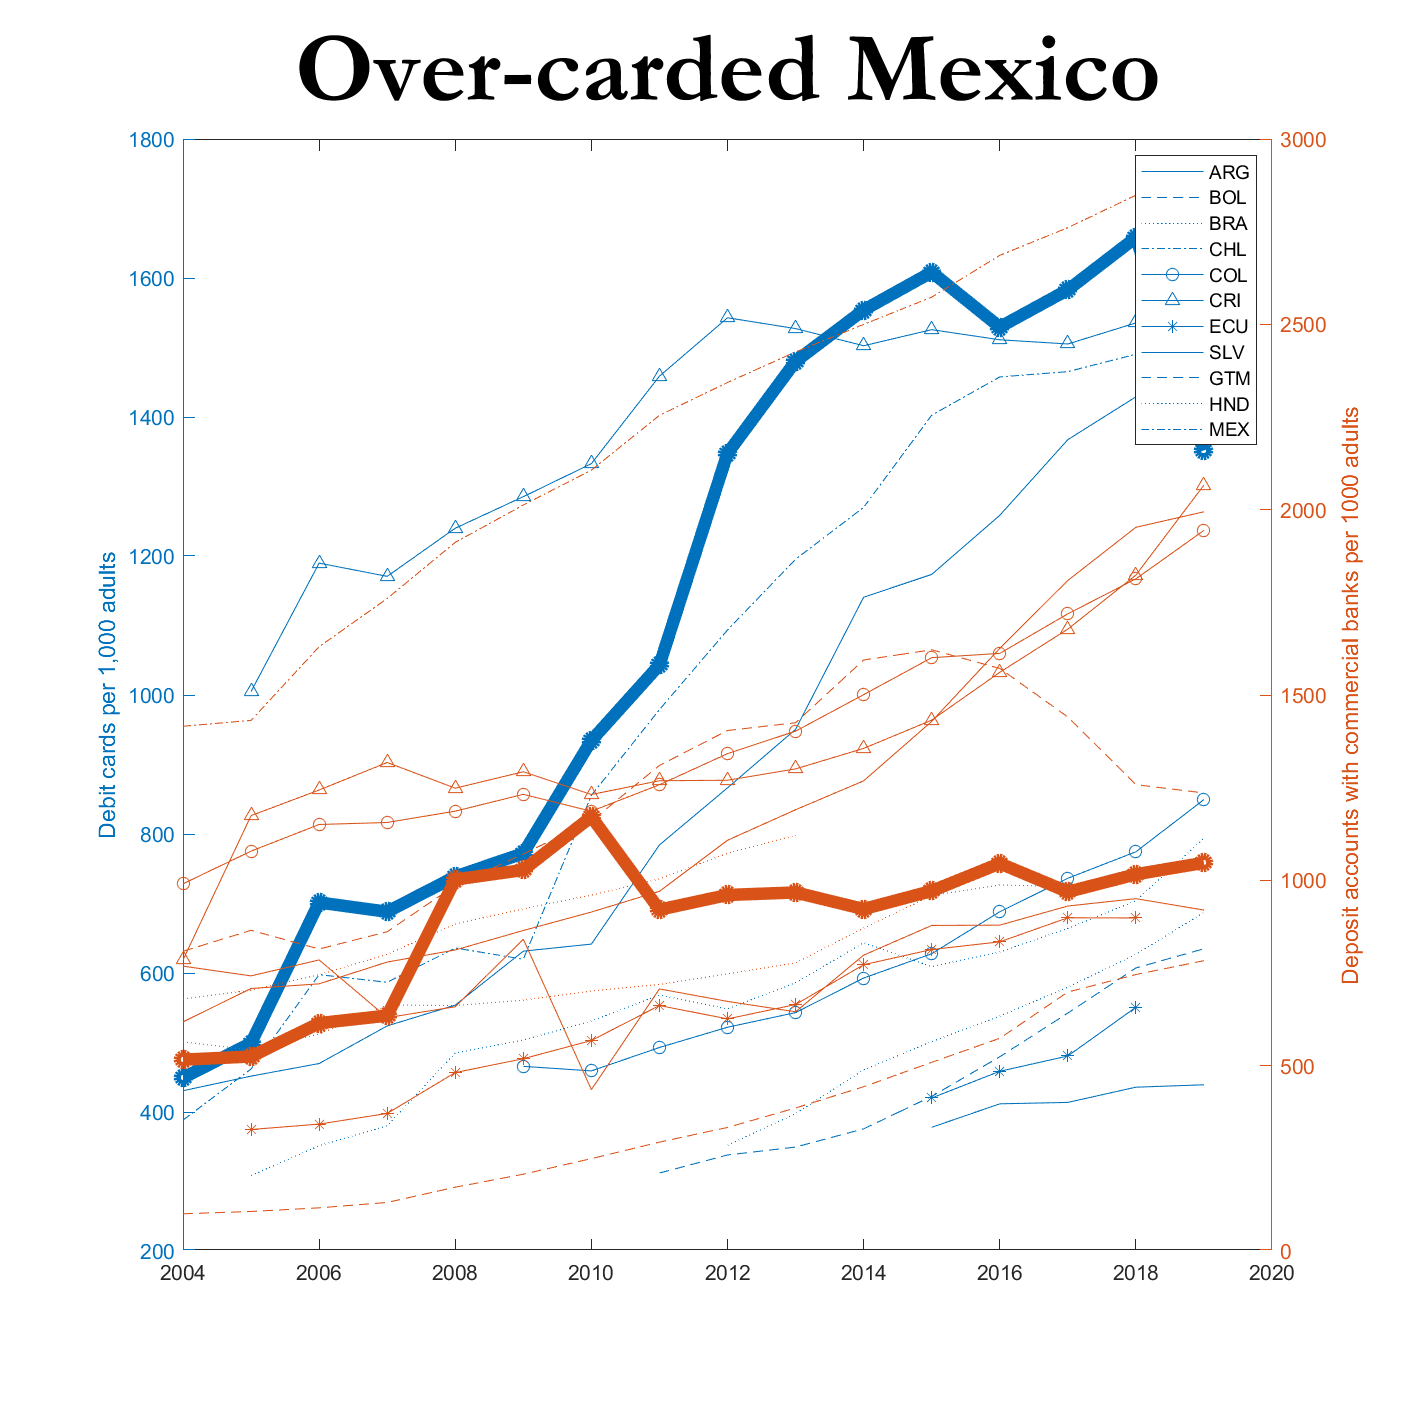
\includegraphics[scale=0.3]{LM_CardsPerDepositBAD}
\par\end{center}

\end{frame}
%
\begin{frame}{Yet another revision}
\begin{center}
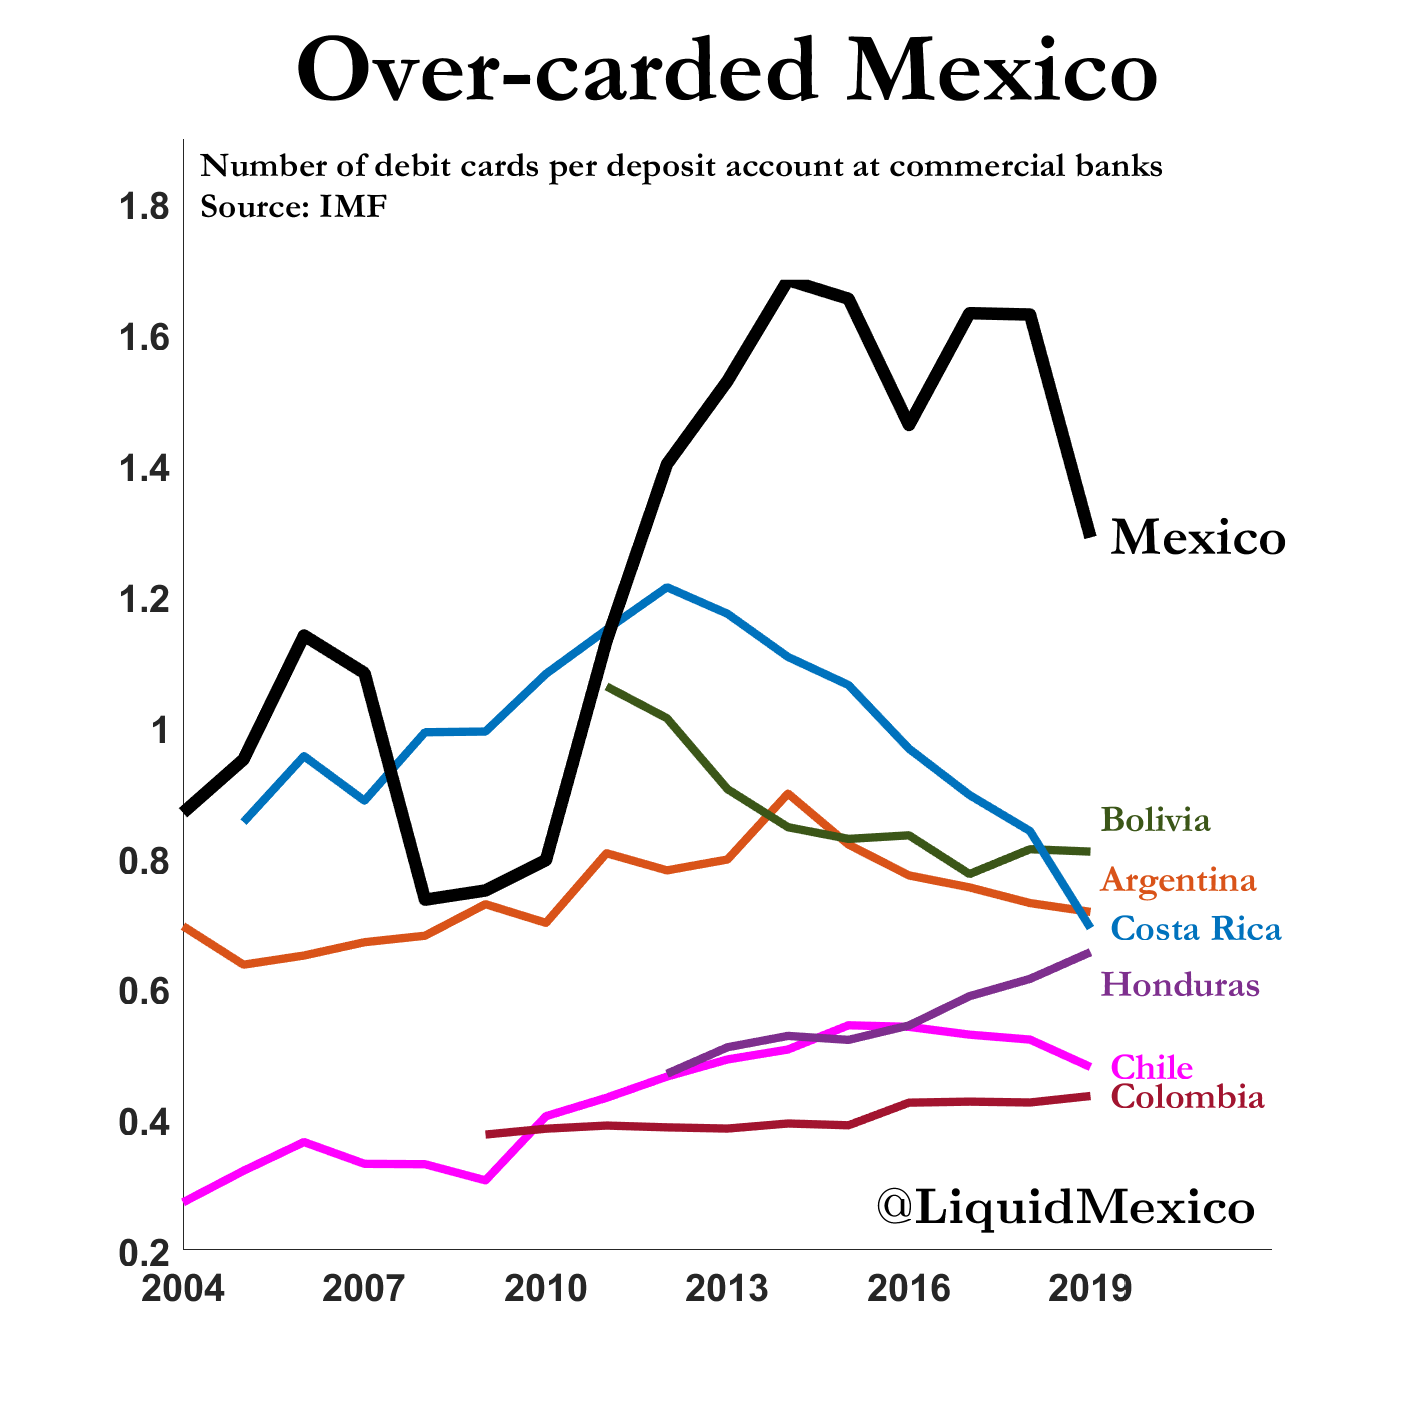
\includegraphics[scale=0.3]{LM_CardsPerDeposit}
\par\end{center}

\end{frame}
%
\begin{frame}{How about this one?}
\begin{center}
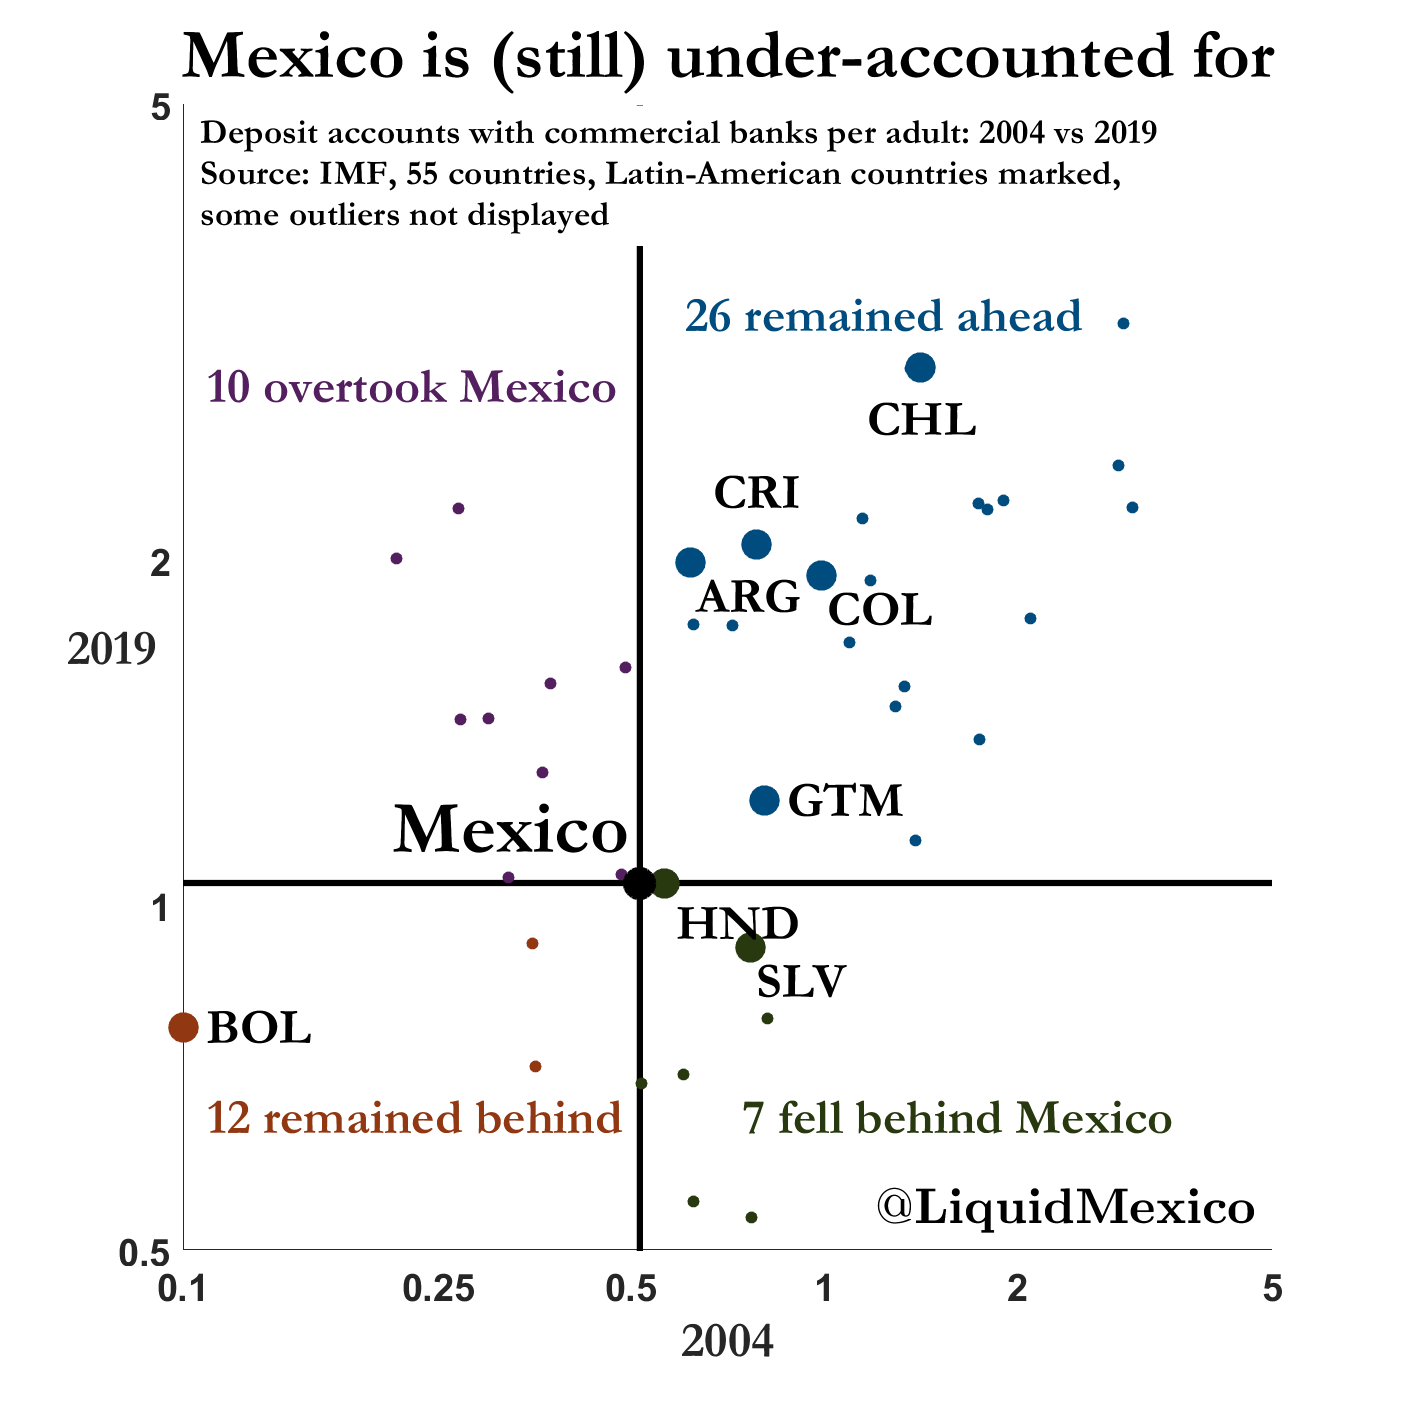
\includegraphics[scale=0.3]{LM_Deposits}
\par\end{center}

\end{frame}
%
\begin{frame}{How about this one?}
\begin{center}
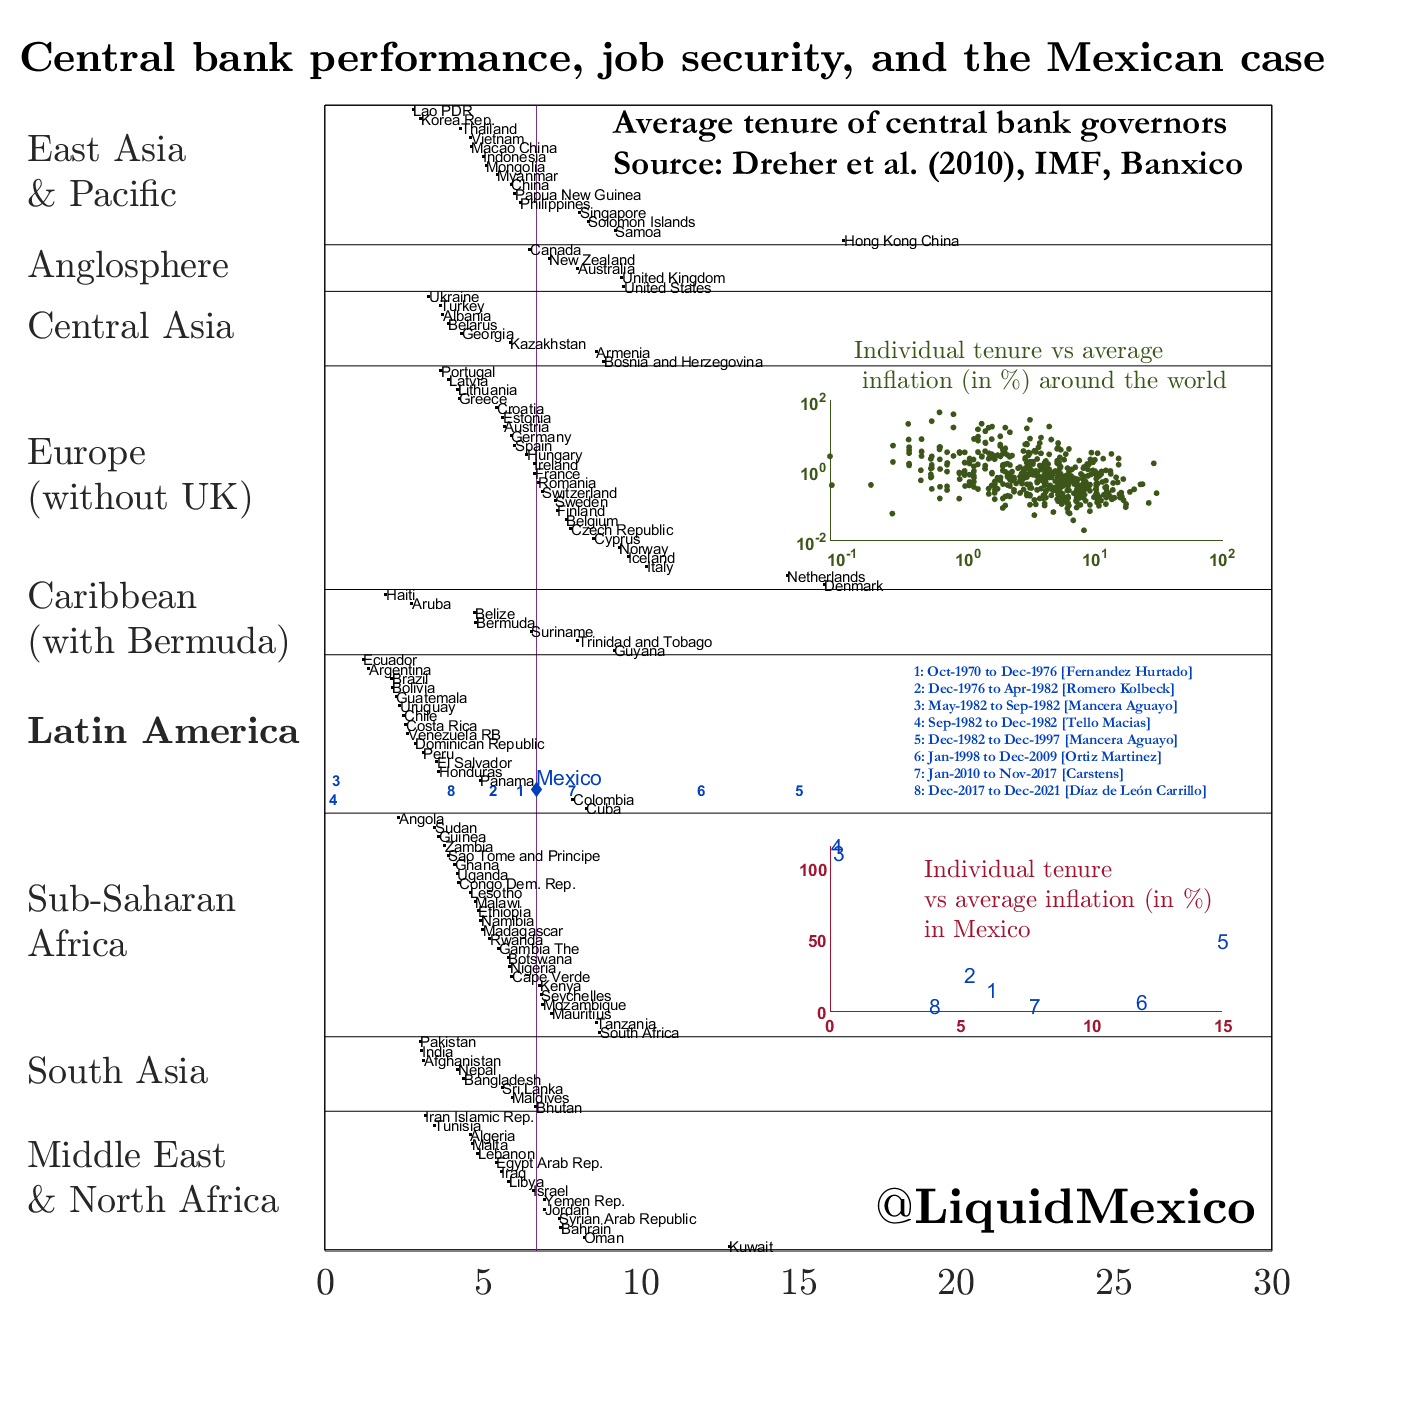
\includegraphics[scale=0.3]{LM_InflationVsTenure}
\par\end{center}

\end{frame}
%
\begin{frame}{How about this one?}
\begin{center}
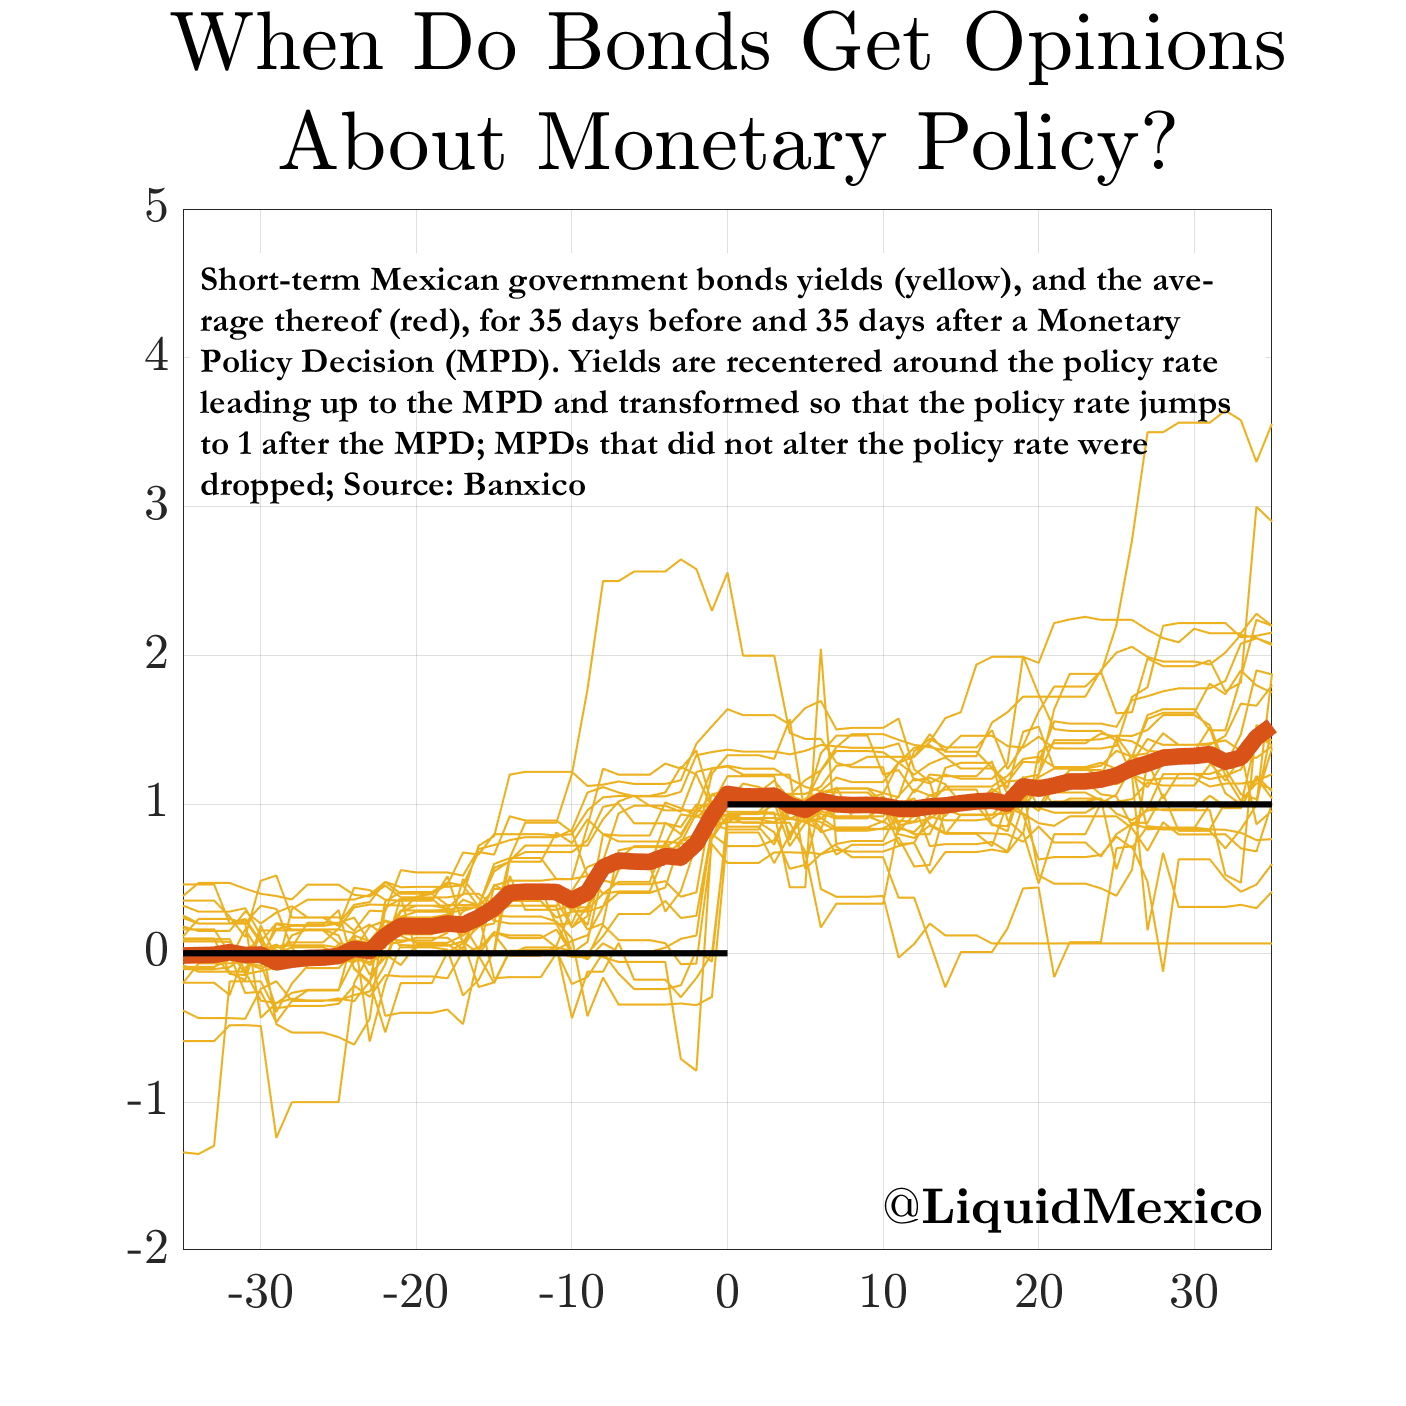
\includegraphics[scale=0.3]{LM_BondsWithOpinions}
\par\end{center}

\end{frame}
%
\begin{frame}{How about this one?}
\begin{center}
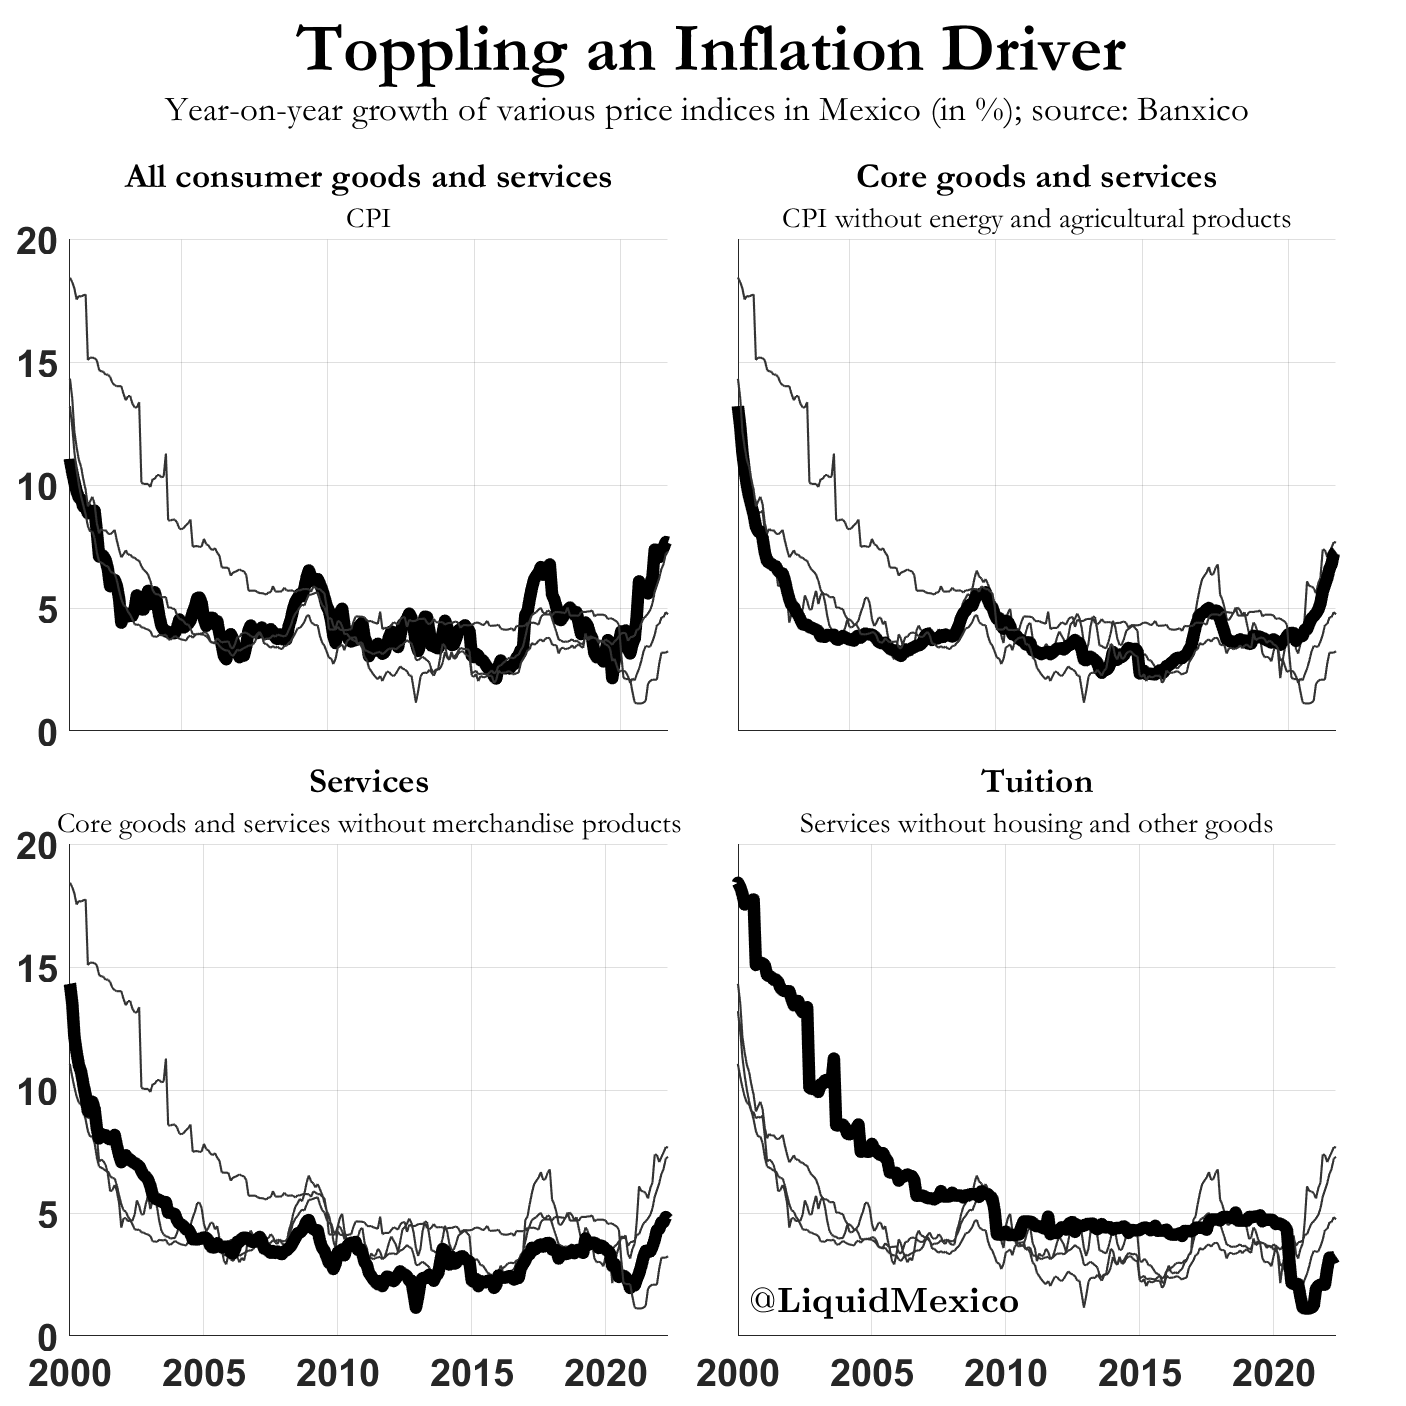
\includegraphics[scale=0.3]{LM_EducationInflation}
\par\end{center}

\end{frame}
%
\begin{frame}{How about this one?}
\begin{center}
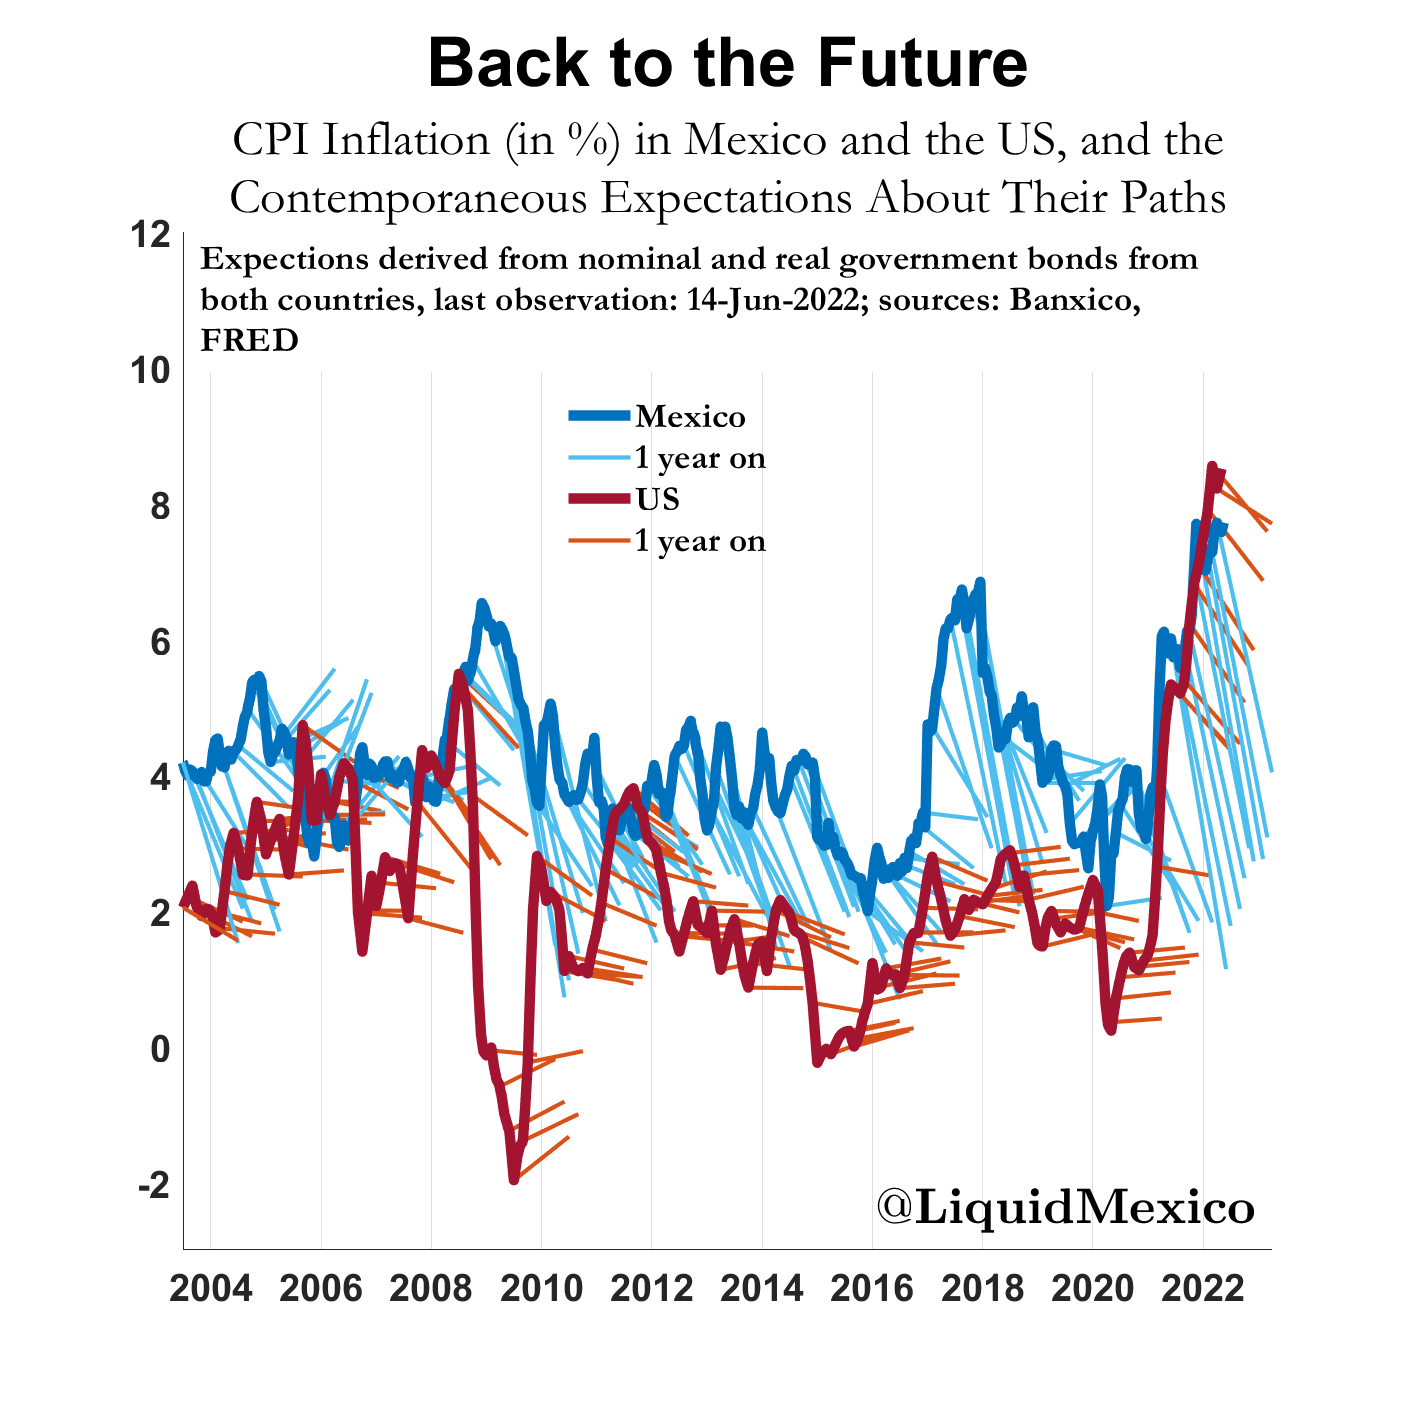
\includegraphics[scale=0.3]{LM_ImpliedInflationExpectations}
\par\end{center}

\end{frame}
%
\begin{frame}{How about this one?}
\begin{center}
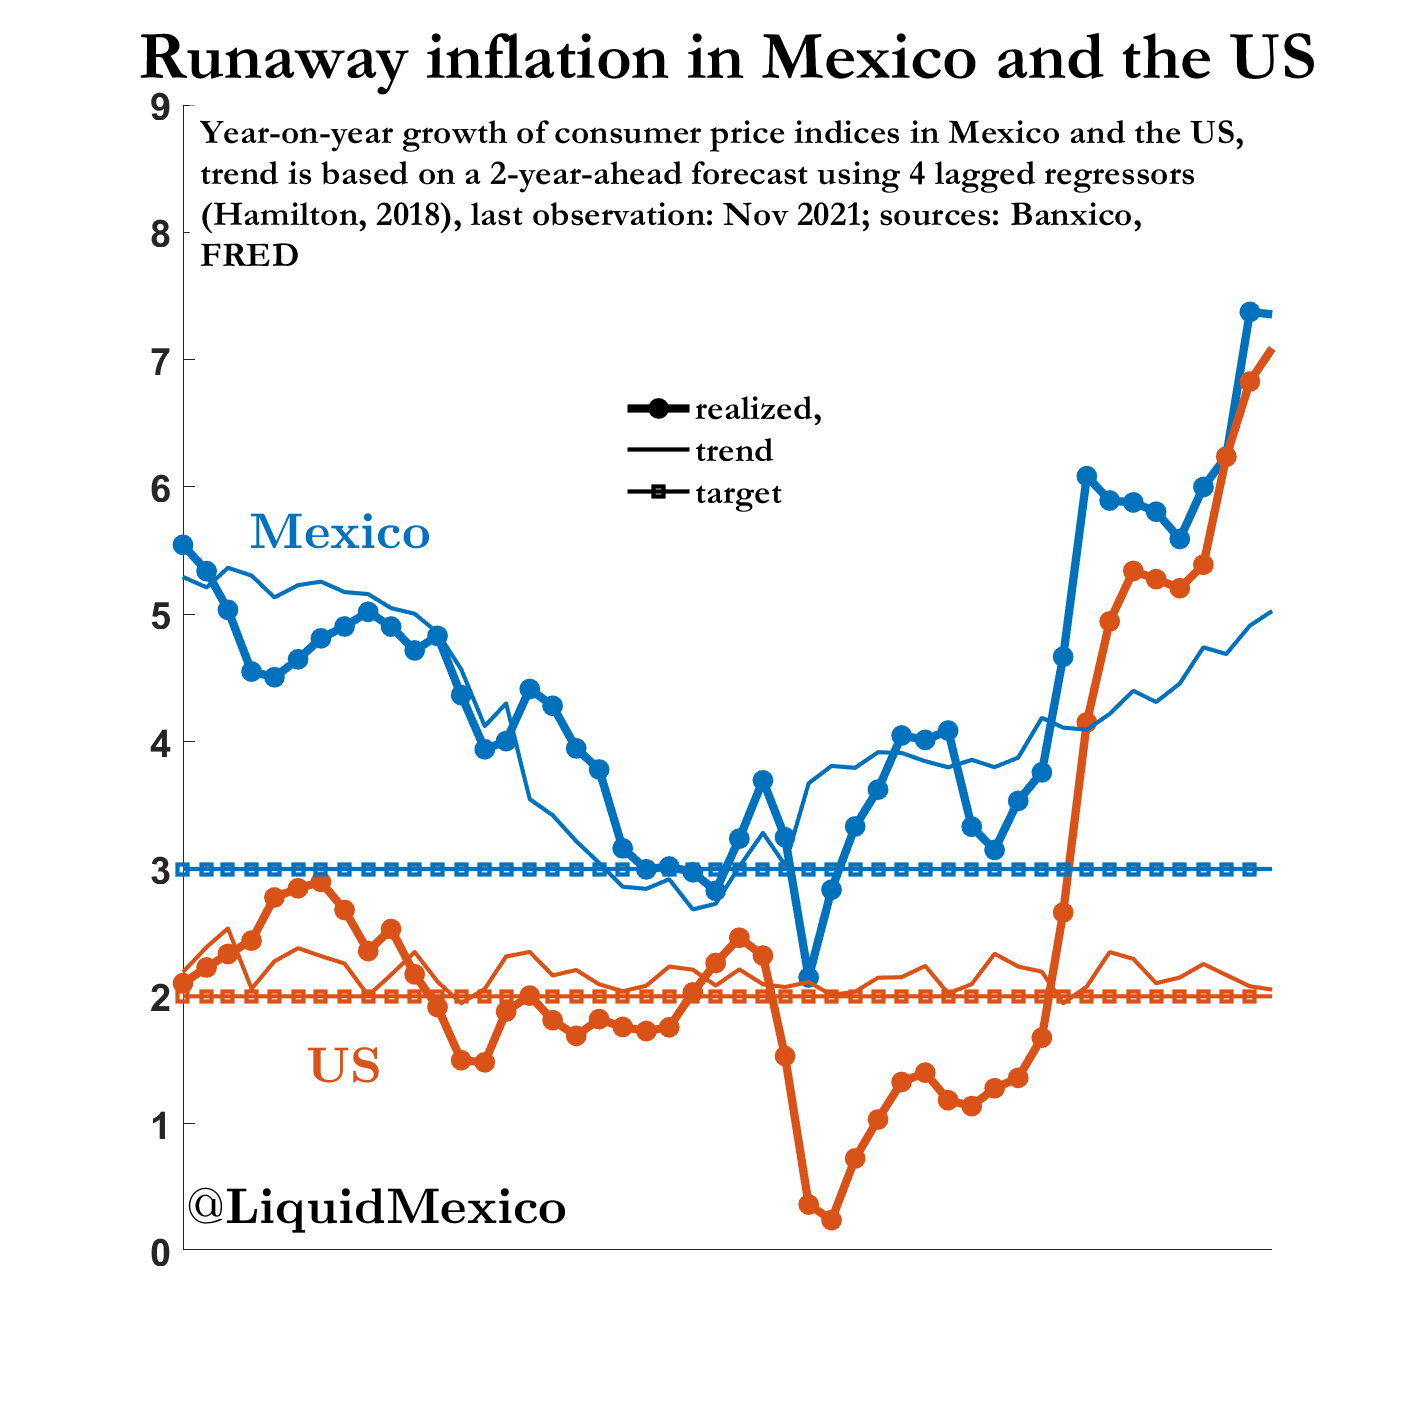
\includegraphics[scale=0.3]{LM_Inflation2021Nov}
\par\end{center}

\end{frame}
%
\begin{frame}{How about this one?}
\begin{center}
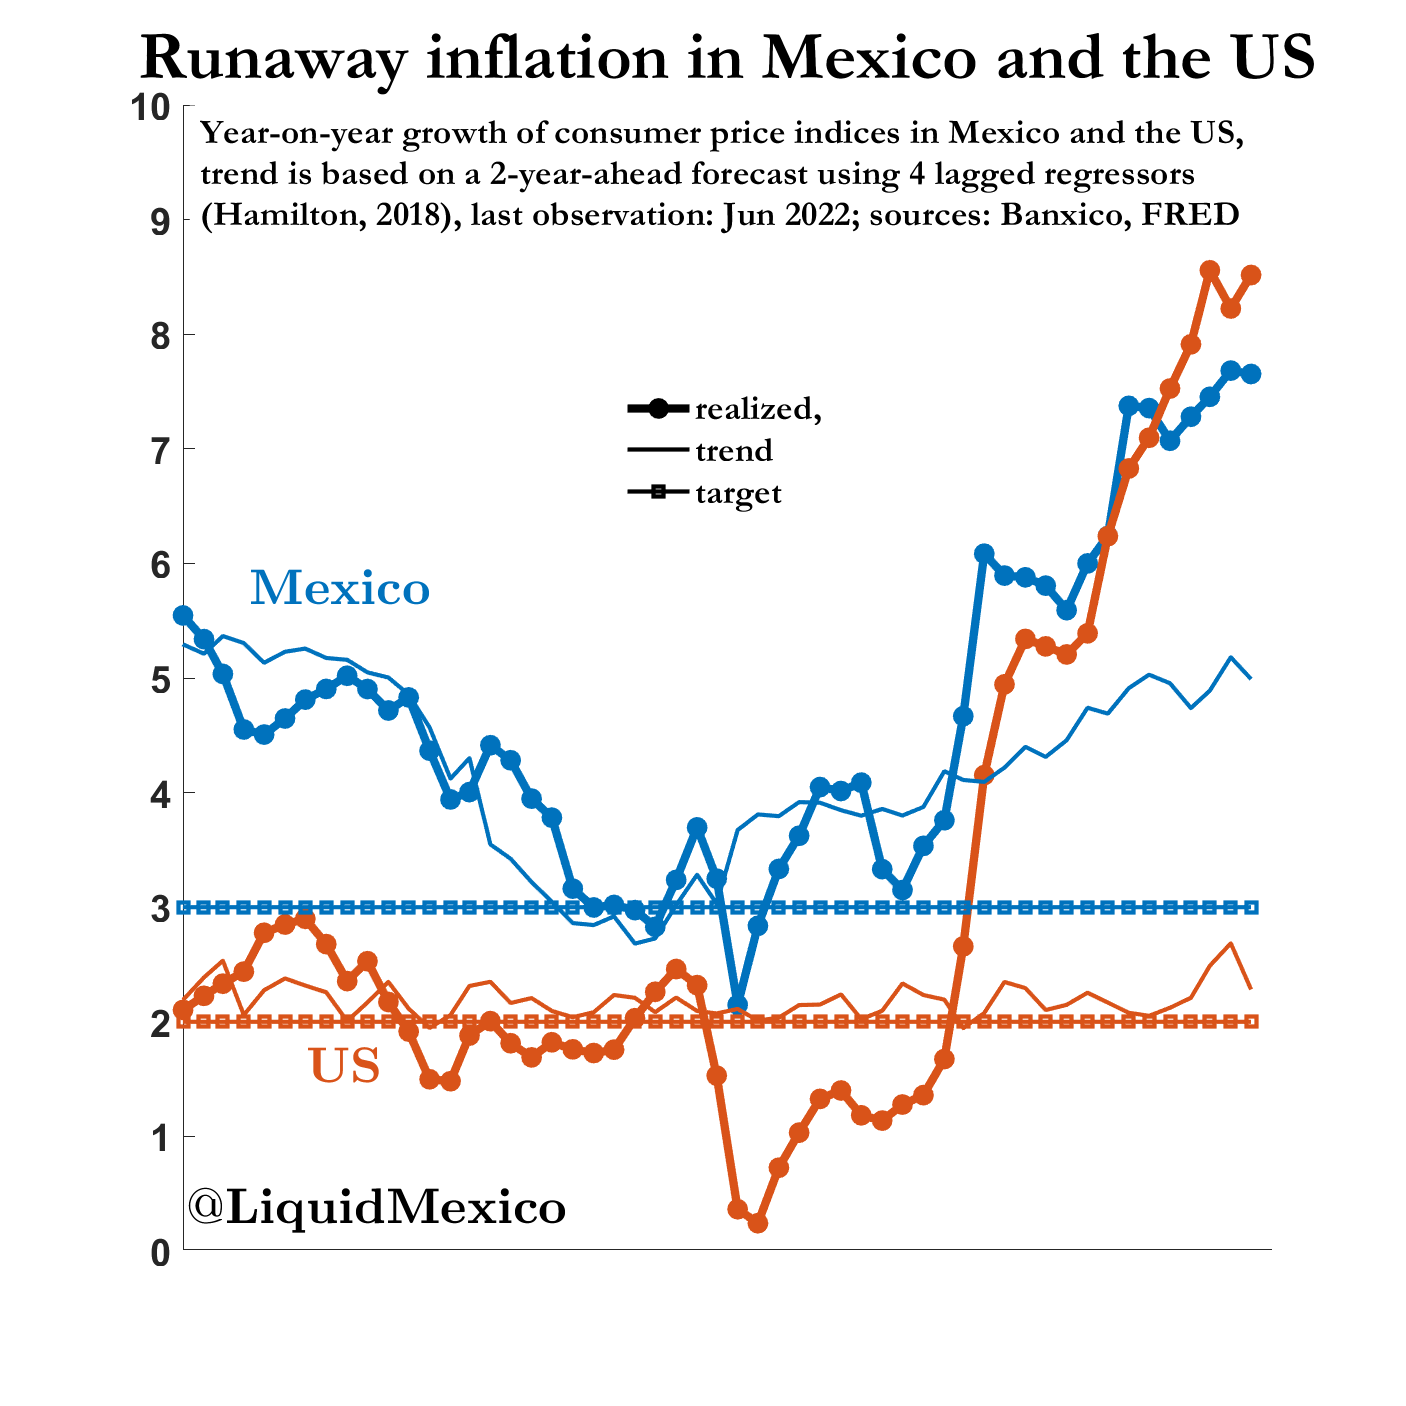
\includegraphics[scale=0.3]{LM_Inflation2022June}
\par\end{center}

\end{frame}
%
\begin{frame}{How about this one?}
\begin{center}
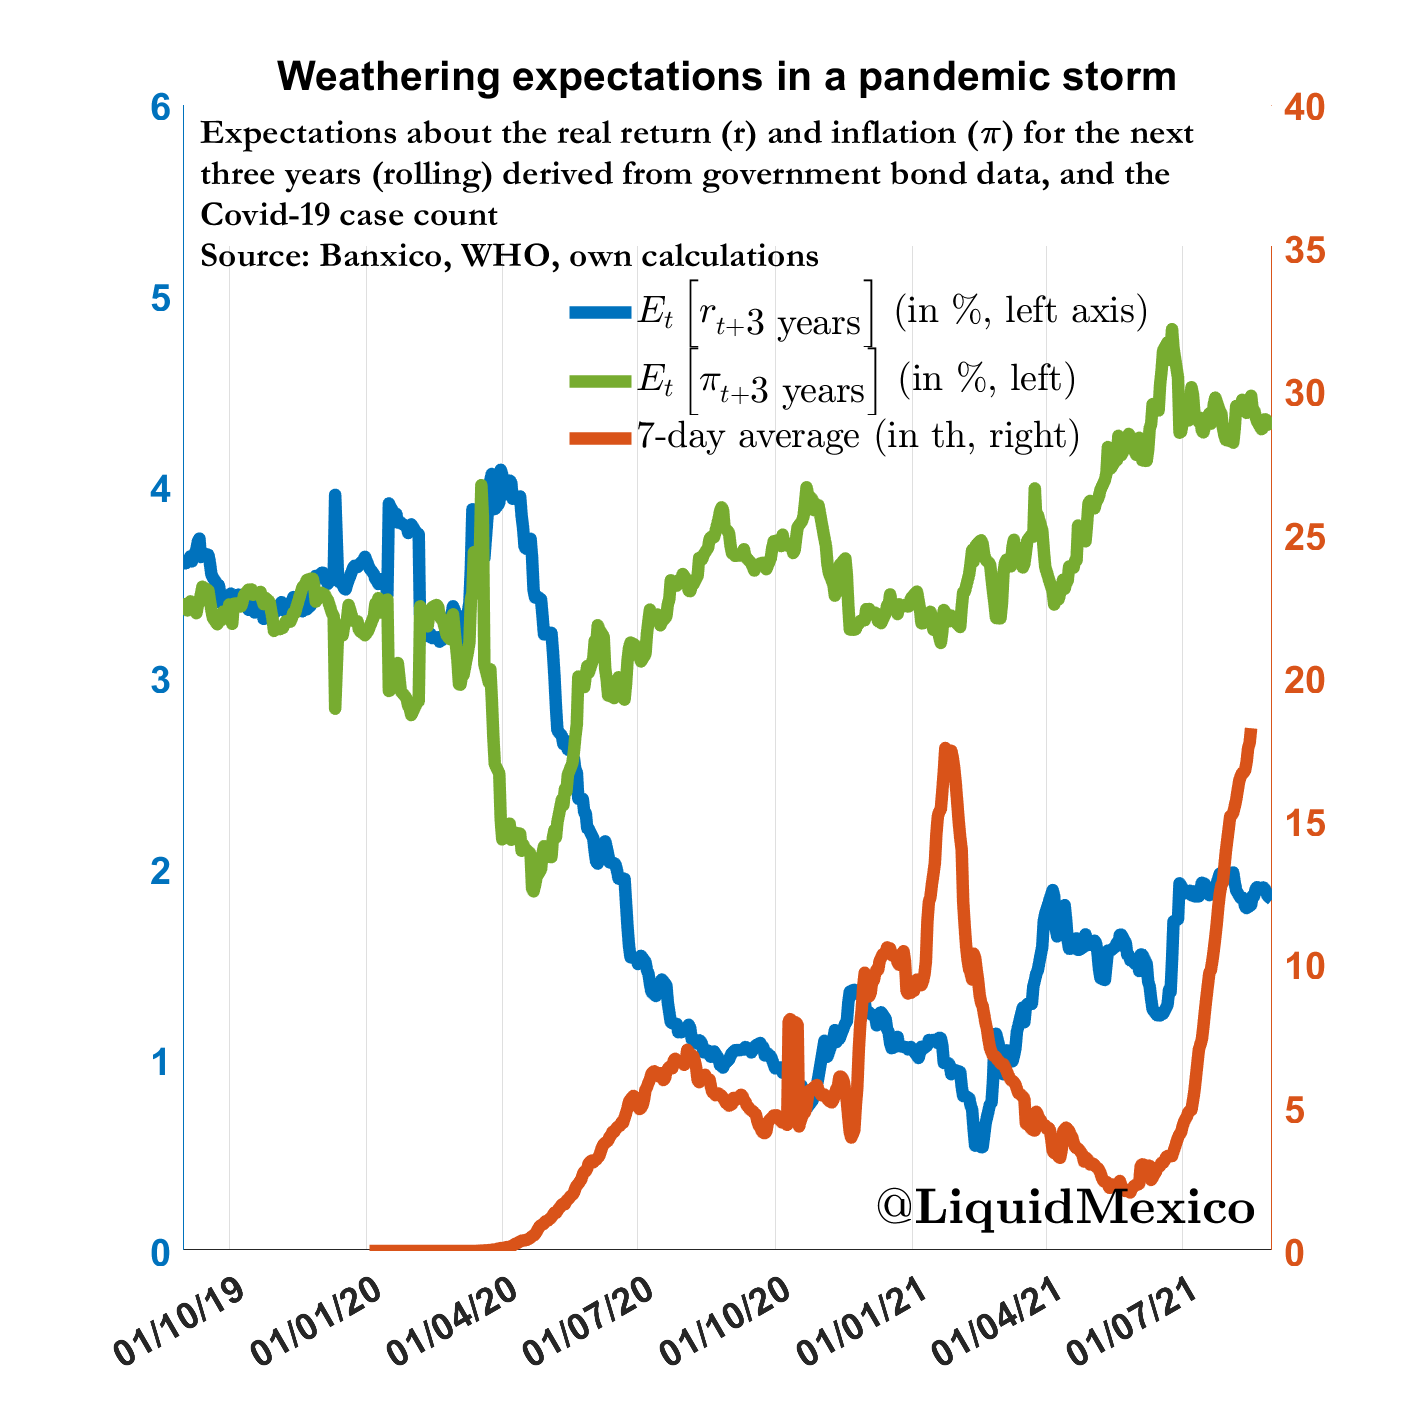
\includegraphics[scale=0.3]{LM_WeatheringAPandemic}
\par\end{center}

\end{frame}
%
\begin{frame}{How about this one?}
\begin{center}
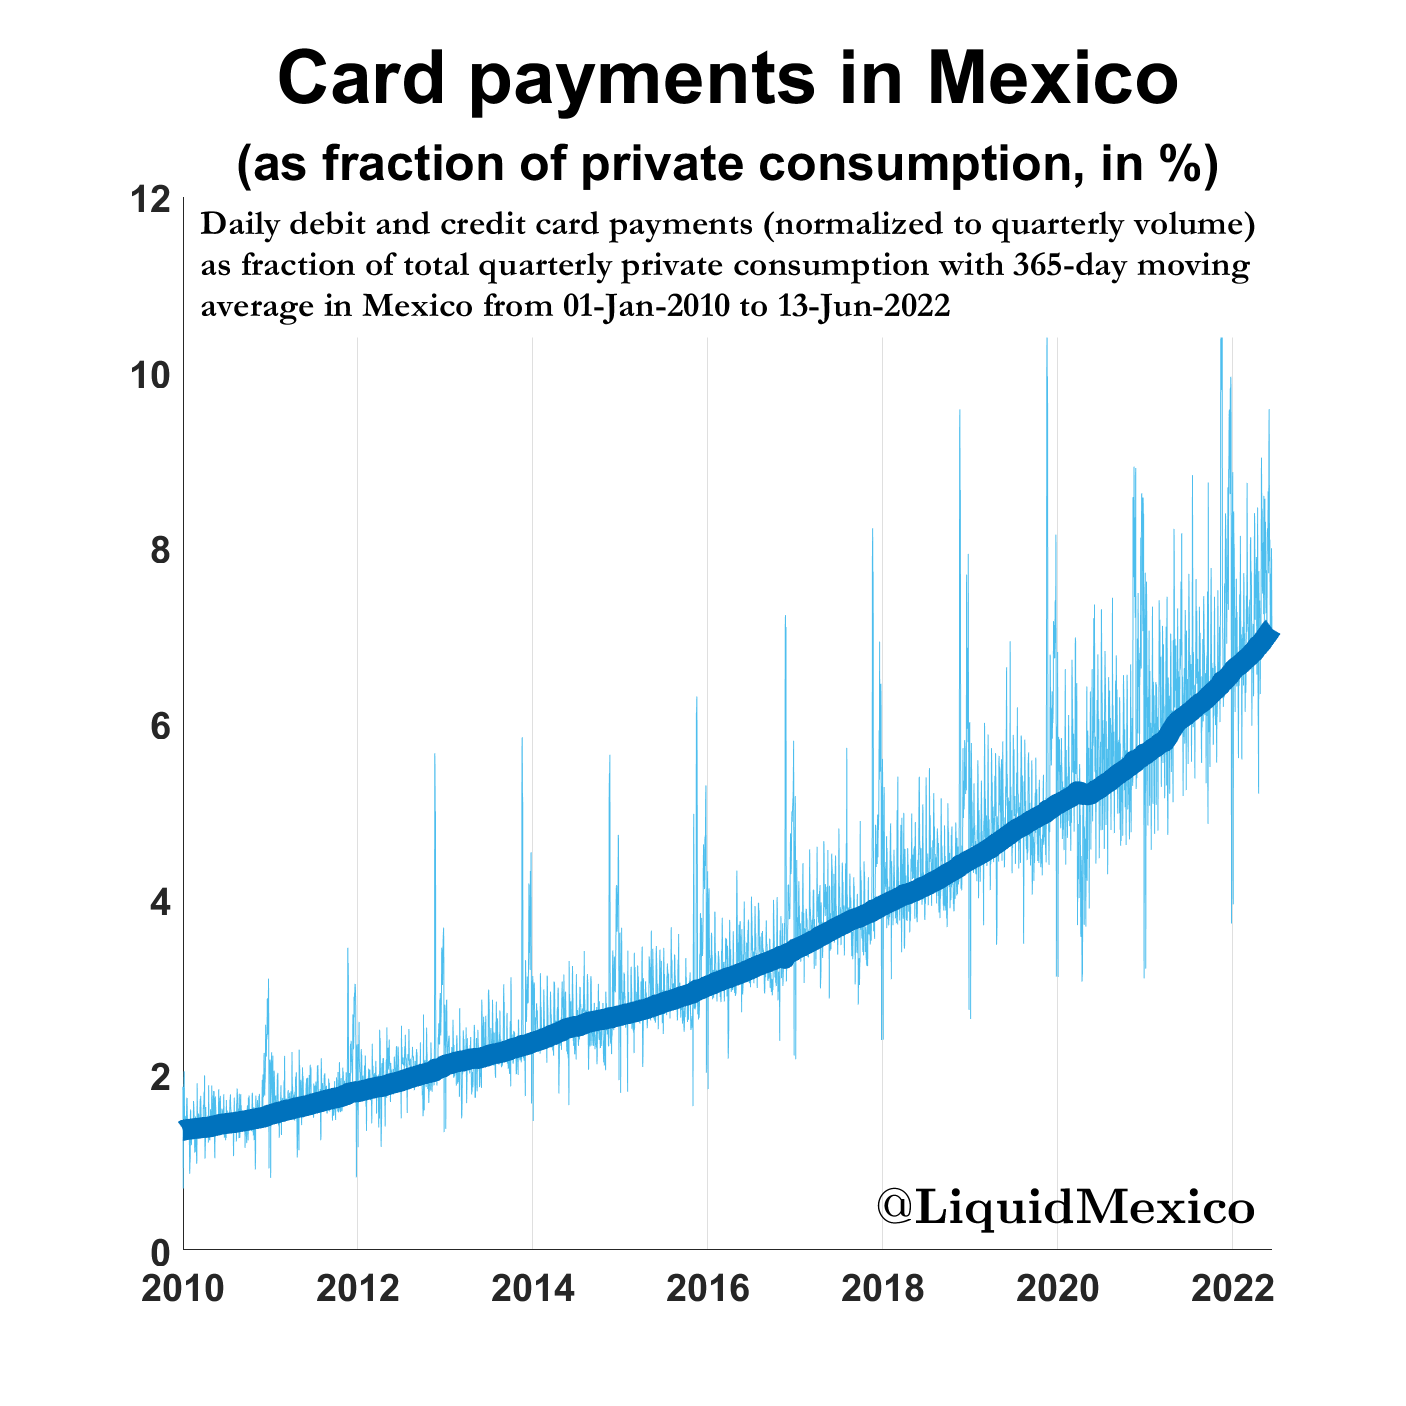
\includegraphics[scale=0.3]{LM_CardPaymentsAsFraction}
\par\end{center}

\end{frame}
%
\begin{frame}{Live data visualization}
\begin{center}
\href{https://sites.google.com/view/alexanderdentler/monitoring-mexico}{Monitoring Mexico}
\par\end{center}

\end{frame}
%
\bibliographystyle{chicago}
\bibliography{\string"../../../Working Papers/library_references/bib_list\string"}

\end{document}
